%! Author = zuffik
%! Date = 02/02/2020

\documentclass[12pt]{article}

% Packages
\usepackage{amsmath}
\usepackage{geometry}
\usepackage[utf8]{inputenc}
\usepackage{mathptmx}
\usepackage[slovak]{babel}
\usepackage{hyperref}
\usepackage{titlesec}
\usepackage[T1]{fontenc}
\usepackage{cite}
\usepackage{listings}
\usepackage{xcolor}
\usepackage{graphicx}
\usepackage{csquotes}
\usepackage{multirow}
\usepackage{regexpatch}
\usepackage{longtable}
\usepackage[notintoc]{nomencl}
\usepackage{verbatim}
\usepackage{comment}
\usepackage{float}
\usepackage{datetime}
\usepackage{pgf,interval}
\usepackage{anyfontsize}

% Document
\graphicspath{ {./images} }
\hypersetup{
    colorlinks,
    citecolor=black,
    filecolor=black,
    linkcolor=black,
    urlcolor=black
}
\geometry{a4paper, portrait, left=3.5cm, right=2cm, top=2.5cm, bottom=2.5cm}
\linespread{1.25}
\title{Záverečná práca}
\author{Kristián Žuffa}
\date{ }

% Renew
\let\bkupitemize\itemize
\let\bkupenditemize\enditemize
\renewenvironment{itemize}{\bkupitemize\addtolength{\itemsep}{-0.3\baselineskip}}{\bkupenditemize}
\let\bkupenumerate\enumerate
\let\bkupendenumerate\endenumerate
\renewenvironment{enumerate}{\bkupenumerate\addtolength{\itemsep}{-0.3\baselineskip}}{\bkupendenumerate}

\newcommand{\sectionbreak}{\clearpage}
\newcommand{\shellcmd}[1]{\texttt{\footnotesize#1}}

\lstset{
  literate={á}{{\' a}}1
           {Á}{{\' A}}1
           {é}{{\' e}}1
           {É}{{\' E}}1
           {í}{{\' i}}1
           {Í}{{\' I}}1
           {ó}{{\' o}}1
           {Ó}{{\' O}}1
           {ú}{{\' u}}1
           {Ú}{{\' U}}1
           {ý}{{\' y}}1
           {Ý}{{\' Y}}1
           {ĺ}{{\' l}}1
           {Ĺ}{{\' L}}1
           {ŕ}{{\' r}}1
           {Ŕ}{{\' R}}1
           {ď}{{\v d}}1
           {Ď}{{\v D}}1
           {ť}{{\v t}}1
           {Ť}{{\v T}}1
           {ň}{{\v n}}1
           {Ň}{{\v N}}1
           {ľ}{{\v l}}1
           {Ľ}{{\v L}}1
           {č}{{\v c}}1
           {Č}{{\v C}}1
           {ž}{{\v z}}1
           {Ž}{{\v Z}}1
           {š}{{\v s}}1
           {Š}{{\v S}}1
}

\makeatletter
% Change the `-` delimiter to an active character
\xpatchparametertext\@@@cmidrule{-}{\cA-}{}{}
\xpatchparametertext\@cline{-}{\cA-}{}{}
\makeatother
\makeatletter
\patchcmd{\thenomenclature}{\section*}{\section}{}{}
\makeatother

\renewcommand{\nomname}{Použité skratky}
\makeatletter
\def\thenomenclature{
  \section*{\nomname}
  \if@intoc\addcontentsline{toc}{section}{\nomname}\fi%
\nompreamble
\list{}{%
\labelwidth\nom@tempdim
\leftmargin\labelwidth
\advance\leftmargin\labelsep
\itemsep\nomitemsep
\let\makelabel\nomlabel}}
\lstset{
    escapeinside={\%*}{*)},
    breaklines=true,
    breakatwhitespace=true,
    extendedchars=false,
    inputencoding=utf8
}
\def\HyLang@slovak{%
  \def\equationautorefname{Equation}%
  \def\footnoteautorefname{footnote}%
  \def\itemautorefname{item}%
  \def\figureautorefname{obrázku}%
  \def\tableautorefname{Table}%
  \def\partautorefname{Part}%
  \def\appendixautorefname{Appendix}%
  \def\chapterautorefname{chapter}%
  \def\sectionautorefname{section}%
  \def\subsectionautorefname{podkapitole}%
  \def\subsubsectionautorefname{podkapitole}%
  \def\paragraphautorefname{paragraph}%
  \def\subparagraphautorefname{subparagraph}%
  \def\FancyVerbLineautorefname{line}%
  \def\theoremautorefname{Theorem}%
  \def\pageautorefname{page}%
}
\g@addto@macro\extrasslovak\HyLang@slovak
\makeatother


\begin{document}
    \nomenclature{$ANN$}{Umelá neurónová sieť (Artificial neural networks)}
\nomenclature{$SVM$}{Metóda podporných vektorov (Support vector machine)}
\nomenclature{$angl.$}{anglicky}
\nomenclature{$skr.$}{skratka}

\pagenumbering{gobble}
\begin{center}
\begin{uppercase}
    {\uppercase{\fontsize{18pt}{0}\selectfont \textbf{Žilinská univerzita v Žiline} \par}}
    \vspace{5mm}
    {\uppercase{\fontsize{18pt}{0}\selectfont Fakulta riadenia a informatiky \par}}
    \vfill
        {\uppercase{\fontsize{24pt}{0}\selectfont Diplomová práca \par}}
    \vfill
\end{uppercase}
{\uppercase{\fontsize{18pt}{0}\selectfont Kristián Žuffa \par}}
\vspace{5mm}
{\fontsize{18pt}{0}\selectfont \textbf{Využitie metód umelej inteligencie pre účely} \par}
\vspace{1mm}
{\fontsize{18pt}{0}\selectfont \textbf{implementácie zvolenej aplikácie do prostredia Cave} \par}
\vspace{5mm}
Vedúci práce: Ing. Katarína Zábovská, PhD.\\
Registračné číslo: 1130/2019\\
Žilina, 2020\\
\end{center}
\pagebreak

\begin{abstract}
ŽUFFA, Kristián: Využitie metód umelej inteligencie pre účely implementácie zvolenej aplikácie do prostredia Cave.
[diplomová práca].
- Žilinská univerzita.
Fakulta riadenia a informatiky, -
Vedúci práce: Ing. Katarína Zábovská, PhD.
Stupeň odbornej kvalifikácie: inžinier.
Študijný program: inteligentné informačné systémy.
Žilina 2020.~\pageref{LastPage} strán.
\\
Táto záverečná pojednáva o analýze rôznych metód umelej inteligencie pre zvolenú konkrétnu implementáciu a to hru
piškvorky hrané v priestore (3d piškvorky).
Pri analýze boli vybraté a implementované 2 metódy: exaktná metóda minimax a umelá neurónová sieť a aplikácia bola
implementovaná do prostredia Unity.
Hra mala byť pripravená pre beh v prostredí Cave no kvôli nedostatku prostriedkov, ktorý bol spôsobený karanténou
súvisiacou s ochorením koronavírus, nebolo možné tento cieľ splniť.
Napriek tomu hra bola implementovaná ako desktopová aplikácia pre všetky komerčné platformy.
\\

ŽUFFA, Kristián: Artificial intelligence methods within the Cave environment game implementation.
[diploma thesis].
- Unifersity of Žilina.
Faculty of Management Science and Informatics, -
Supervisor: Ing. Katarína Zábovská, PhD.
Qualification: master.
Study program: intelligent information systems.
Žilina 2020.~\pageref{LastPage} pages.
\\
This thesis deals with analysis of different artificial intelligence methods for chosen specific implementation which
is the Tic-Tac-Toe game played in space (3d tic-tac-toe).
There were 2 methods analyzed and implemented: minimax exact method and artificial neural network and the game was
implemented in Unity.
The game was supposed to be ready to run in Cave environment but due to insufficient resources, caused by quarantine
related to corona virus, this target was not completed.
Despite that the game was implemented as desktop application for all commercial platforms.
\\


\end{abstract}
\tableofcontents

\listoffigures
\listoftables
\printnomenclature
\pagebreak
\pagenumbering{arabic}
\setcounter{page}{6}

    \section{Umelá inteligencia}\label{sec:ai}

Od počiatku vzniku mechanických strojov, ktoré pomáhajú ľuďom pri svojej práci sa pri nich nepriamo niesol aj pojem
"umelá inteligencia".
Medzi odbornou verejnosťou tento pojem stále nie je jednotný, no väčšina z nich má rovnakú myšlienku:
inteligencia vykonávaná strojmi (narozdiel od prirodzenej inteligencie, ktorú vykonávajú ľudia, či zvieratá).
Ak stroj (aj mechanický) dokáže niečo vykonať bez explicitného príkazu, je považovaný za inteligentný.

\subsection{Metódy}\label{subsec:ai-methods}

Umelá inteligencia (angl. artificial intelligence) je široká vedná disciplína, ktorá zahŕňa
\begin{itemize}
    \item strojové učenie
    \item textovú analýza
    \item analýzu reči
    \item prevod textu na reč
    \item expertné systémy
    \item plánovanie
    \item optimalizáciu
    \item robotiku
    \item analýzu obrazu
    \item a mnoho ďalšieho
\end{itemize}
Metódy niektorých skupín sa môžu prelínať (napr. na analýzu obrazu a na analýzu zvuku sa môžu použiť umelé neurónové
siete).
Dôsledkom toho je aj fakt, že niektoré metódy sa používajú viac a iné menej.
Nižšie sú popísané metódy, ktoré sú v rámcu umelej inteligencie využívané najlepšie.

\subsubsection{Heuristické metódy}

Heuristiky sú často používanou metódou vo vyhľadávacích algoritmoch.
Na rozdiel od exaktných algoritmov, ktoré prehľadávajú celý vyhľadávací priestor, heuristiky prehľadávajú len okolie
východiskového riešenia.
Ak napríklad je cieľom heuristiky nájsť minimum nejakej funkcie (nemusí byť zadaná analyticky) v $n$-rozmernom priestore,
dokáže táto metóda nájsť len lokálne minimum závislé na tom, kde sa nachádza východzie riešenie.
Príklad je uvedený pre funkciu
\begin{equation}
    f(x,y)=e^{\cos(x)+\sin(y)}\frac{x+y}{30}+\frac{5}{2}
\end{equation}
kde $x\in<-12,12>$, $y\in<-12,12>$.
\begin{figure}[H]
    \centering
    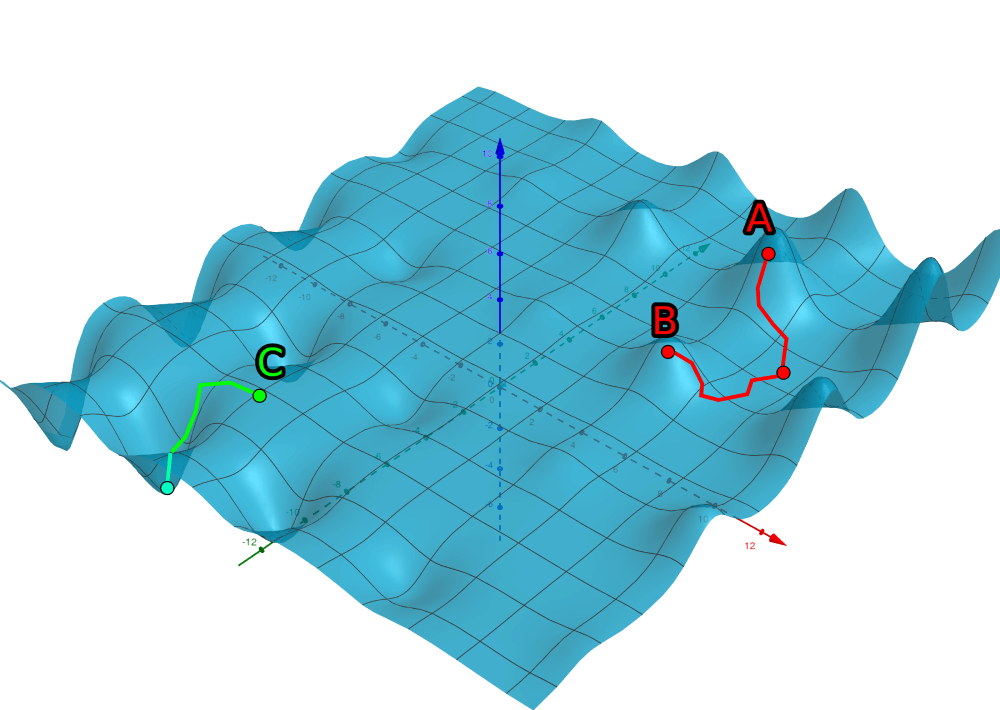
\includegraphics[width=0.8\textwidth]{images/heuristic.png}
    \caption{Heuristika a jej riešenia v závislosti od východzieho riešenia}
\end{figure}\label{figure:heuristic-method}
Pri nastavení východiskového bodu \textbf{A} alebo \textbf{B} nájde heuristika rovnaké lokálne minimum (čo sa môže javiť
ako globálne), no pre východzí bod \textbf{C} nájde algoritmus globálne minimum, čo ale nie je možné overiť bez
prehľadania celého priestoru riešení.
Z toho je možné usúdiť, že riešenie heuristiky nie je vždy optimálne a nikdy jeho optimálnosť nie je zaručená, ale na
druhú stranu sú heuristiky extrémne rýchle.
Heuristické metódy patria medzi najzákladnejšie techniky v rámci umelej inteligencie.

Ako ukážkový príklad praktického využitia heuristických metód je možné uviesť hľadanie najkratšej (alebo najrýchlejšej)
cesty medzi dvoma mestami v cestnej sieti Slovenska pre navigačné systémy alebo pohyb neovládaných postáv v hrách
(angl. non-player character, skr. NPC - akákoľvek postava v hre, ktorú neovláda človek).
Pre oba tieto príklady je možné použiť napríklad \emph{A* algoritmus}.

\subsubsection{Metóda podporných vektorov}

Anglicky support vector machine (skr. SVM) je metóda strojového učenia s učiteľom (reinforcement learning).
Cieľom tejto metódy je nájsť takú \emph{nadrovinu} v $n$-rozmernom vyhľadávacom priestore, ktorá vstupné dáta rozdelí
do dvoch podpriestorov.
Metóda je určená pre klasifikáciu a regresnú analýzu.
Ak je metóda konštruovaná ako optimalizačná úloha jej účelová funkcia vyzerá podobne ako nasledovná:
\begin{equation}
    \max \sum_{\forall i}{\sqrt{\sum_{\forall j}{(\vec{v}_j - x_{ij})^2}}}
\end{equation}
Kde $\vec{v}$ je hľadaný vektor a $\vec{v}_j$ sú jeho zložky a kde $x_i$ je vzorka zo vstupných dát a $x_{ij}$ sú jeho
zložky.
Keďže výraz $\sqrt{\sum_{\forall j}{(\vec{v}_j - x_{ij})^2}}$ vyjadruje najmenšiu vzdialenosť medzi vektorom a
vzorkou, dá sa povedať, že metóda hľadá takú nadrovinu, ktorá vyhľadávací priestor rozdelí čo najlepšie.
\begin{figure}[H]
    \centering
    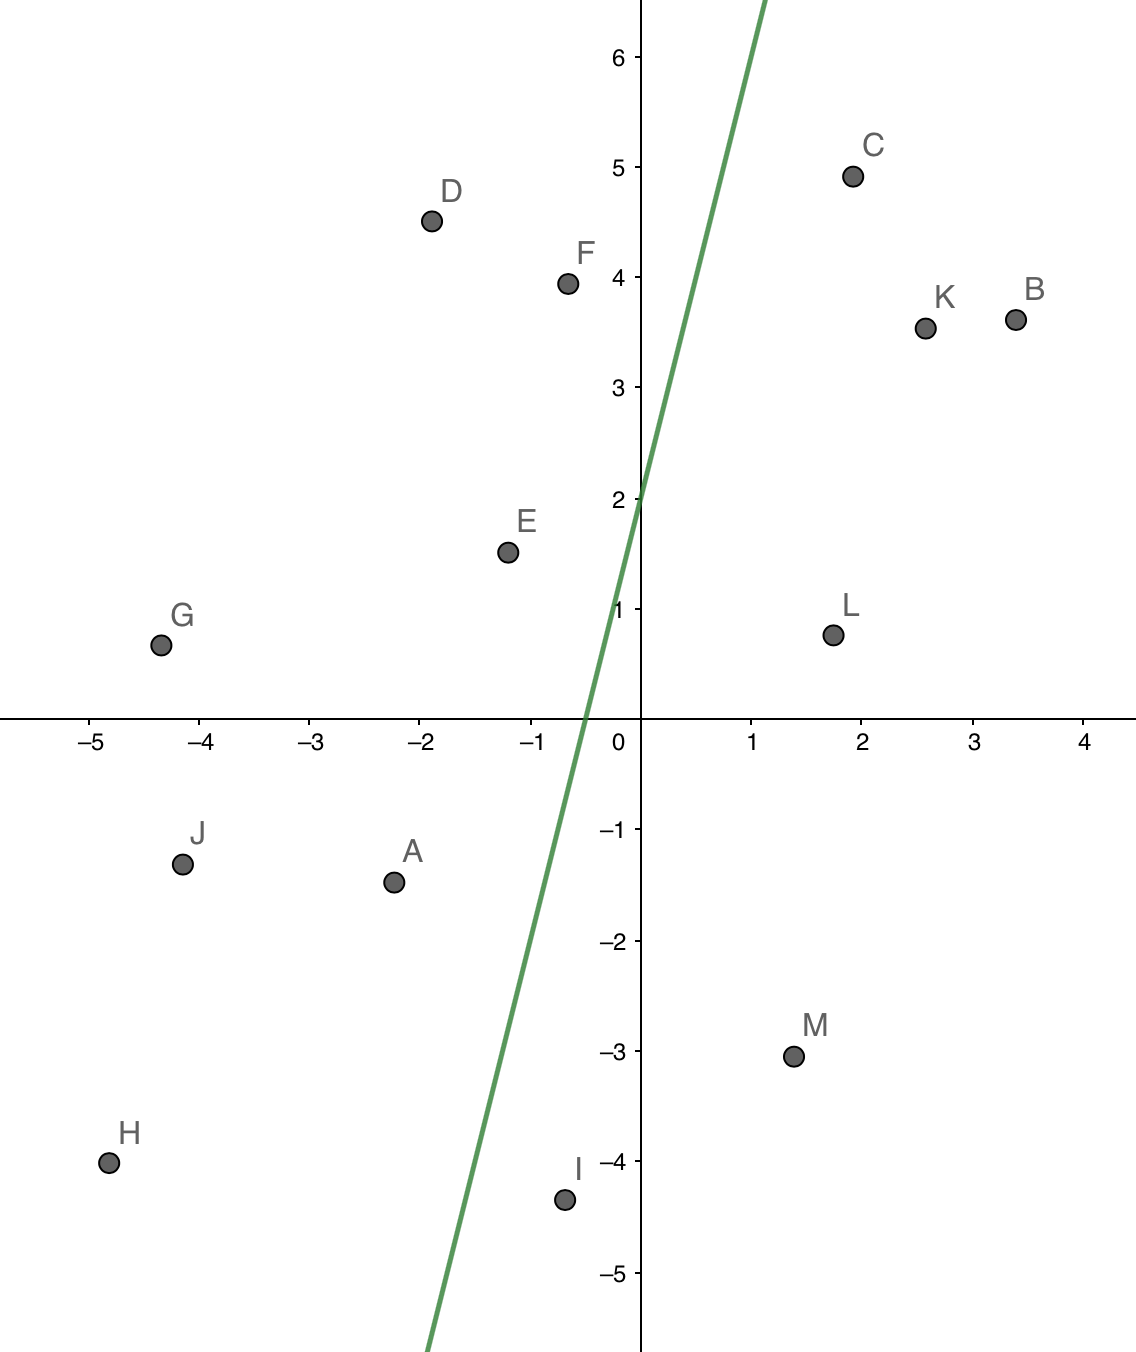
\includegraphics[width=0.5\textwidth]{images/svm.png}
    \caption{Support vector machine}
\end{figure}\label{figure:svm}

Typickým príkladom použitia metódy podporných vektorov je rozdelenie e-mailovej komunikácie do dvoch skupín: relevantnú
a nevyžiadanú poštu, no podporné vektory sa dajú použiť aj na spracovanie obrazu, či textu.

\subsubsection{Iné metódy}

Pre umelú inteligenciu existuje veľké množstvo algoritmov a ich alternatív, z ktorých sú ešte často používané
\emph{umelé neurónové siete}, ktoré sú bližšie popísané v \autoref{subsec:algo-ann} a ako rozhodovacie pravidlo v
teórii hier je často využívaný algoritmus \emph{minimax} (viac v \autoref{subsec:algo-minmax}).

    \section{Návrh riešenia}\label{sec:algorithms}

Počas vývoja výpočtovej techniky sa vyvíjali aj algoritmy pre kombinatorické hry, pričom piškvorky sú jednou z nich.
Tieto algoritmy je možné rozdeliť do 2 skupín: \emph{exaktné} a \emph{heuristické}; v tejto kapitole je popísaný jeden
algoritmus z každej skupiny.

\subsection{MiniMax}\label{subsec:algo-minmax}

Minimax je rozhodovacie pravidlo založený na vyhľadávacom algoritme v strome, podľa ktorého je možné určiť nasledujúci
ťah.\cite{algo_minimax}
Jeho princíp spočíva v maximalizovaní úžitku pre cieľového hráča a minimalizovaní úžitku pre oponenta.
Pôvodne bol vyvinutý pre \emph{hru s nulovým súčtom} (angl. zero-sum), čo je termín používaný v teórii hier.
Vyjadruje hru, kde rozhodnutia hráčov sa dajú ohodnotiť nenulovým číslom $v$, pričom súčet za sebou idúcich hier má
súčet približne 0.
Často používaná hodnota je $v=1$ alebo $v=10$.
Ťah cieľového hráča je vyjadrený kladnou hodnotou ($+v$), ťah protihráča je vyjadrený zápornou hodnotou ($-v$) a remíza
je vyjadrená hodnotou $0$.
Hru, ktorú hrajú hráči striedavo, je možné vyjadriť pomocou postupnosti pre remízu:
\begin{equation}
    v-v+v-v+ \dots = \sum{v-v} = \sum{0} = 0
\end{equation}
(z čoho vychádza aj názov \emph{hra s nulovým súčtom}), resp. pre výhru jedného z hráčov:
\begin{equation}
    \pm v+v-v+v-v+ \dots = \pm v+\sum{v-v} = \pm v+\sum{0} = \pm v
\end{equation}
Rozhodovanie vychádza práve z tohto faktu, pričom algoritmus sa snaží nájsť takú postupnosť ťahov, ktorá by bola rovná
$+v$ (resp. maximálna), čo by znamenalo výhru cieľového hráča.
Samotný rozhodovací proces sa dá vyjadriť pomocou rozhodovacieho stromu vychádzajúceho z ktoréhokoľvek stavu hry.
Stavy hry tvoria vrcholy stromu a hrany predstavujú prechody medzi týmito stavmi.
Stav hry sa dá vyjadriť pomocou $d$-rozmernej tabuľky, kde hodnoty predstavujú \textbf{X}, \textbf{O} alebo prázdne
políčko.

Nech $l$ je maximálna výška rozhodovacieho stromu.
Ak nie je explicitne zadaná, potom maximálna výška stromu je počet voľných políčok vo východiskovom stave hry.
Nech $S_{ij}$ je stav hry, kde $i$ je úroveň stromu, v ktorom sa stav hry nachádza a $j$ je poradové číslo tohto vrcholu
v rámci úrovne $i$ určené pre jednoznačnú identifikáciu stavu hry a nech $p(S_{ij})$ je v strome rodič stavu $S_{ij}$
potom $\forall i, k, j \colon p(S_{i+1,k}) = S_{ij} \colon S_{i+1,k}$ vznikne vyplnením postupne každého
prázdneho políčka znakom hráča, ktorý je na ťahu na úrovni $i$.

Pre lepšiu predstavu je možné si situáciu ukázať na príklade z \hyperref[figure:minimax-tree]{nasledujúceho obrázku}.
Koreň stromu obsahuje 3 voľné políčka, jeho synovia vzniknú vyplnením postupne každého voľného políčka znakom hráča na
úrovni 2 (tzn. \textbf{X} na pozície 1. riadok, druhý stĺpec; tretí riadok, prvý stĺpec a tretí riadok, tretí stĺpec).
Takto sa naplní celý strom a jeho listy sa ohodnotia hotnotami $v$ pre víťazný stav hry, $-v$ pre prehru a $0$ pre
remízu (na \hyperref[figure:minimax-tree]{obrázku} vyznačené čiernou farbou).

Nech
\begin{equation}
    V(S_{ij}) =
    \begin{cases}
        \min{\{V(S_{i+1,j}) \forall j\}} & \text{ak v ťahu } i \text{ je na ťahu protihráč} \\
        \max{\{V(S_{i+1,j}) \forall j\}} & \text{ak v ťahu } i \text{ je na ťahu cieľový hráč}
    \end{cases}
\end{equation}
potom $\forall S_{ij}$ je priradená hodnota $V(S_{ij})$ pre $i = 1 \dots l-1$ a $\forall j$.
Najlepší ťah je potom určený spôsobom
\begin{equation}
    S_{Best} = \max{\{V(S_{2j}) \forall j \colon p(S_{2j}) = S_{11}\}} = \max{\{V(S_{2j}) \forall j\}}
\end{equation}
Vyhľadávanie prebieha potom nasledovne:\cite{algo_minimax_pseudocode}
\begin{tiny}
    \begin{lstlisting}[language=Python]
def minimax(hraciaPlocha, int maximalnaHlbka, bool maximalizacia):
    if maximalnaHlbka = 0 or %*hraciaPlocha nemá žiaden dostupný možný ťah*):
        return hodnota hracej plochy
    if maximalizacia:
        najlepsiaHodnota = -$\infty$
        for %*všetky dostupné ťahy v hracej ploche*):
            novaHraciaPlocha = %*vykonaj ťah v hraciaPlocha*)
            aktualnaHodnota, aktualnyTah = minimax(novaHraciaPlocha, maximalnaHlbka - 1, false))
            if aktualnaHodnota > najlepsiaHodnota:
                najlepsiaHodnota := aktualnaHodnota
                najlepsiTah = aktualnyTah
        return najlepsiaHodnota, najlepsiTah
    else:
        najlepsiaHodnota = $\infty$
        for %*všetky dostupné ťahy v hracej ploche*):
            novaHraciaPlocha = %*vykonaj ťah v hraciaPlocha*)
            aktualnaHodnota, aktualnyTah = minimax(novaHraciaPlocha, maximalnaHlbka - 1, true))
            if aktualnaHodnota < najlepsiaHodnota:
                najlepsiaHodnota := aktualnaHodnota
                najlepsiTah = aktualnyTah
        return najlepsiaHodnota, najlepsiTah
\end{lstlisting}
\end{tiny}

\begin{figure}[H]
    \centering
    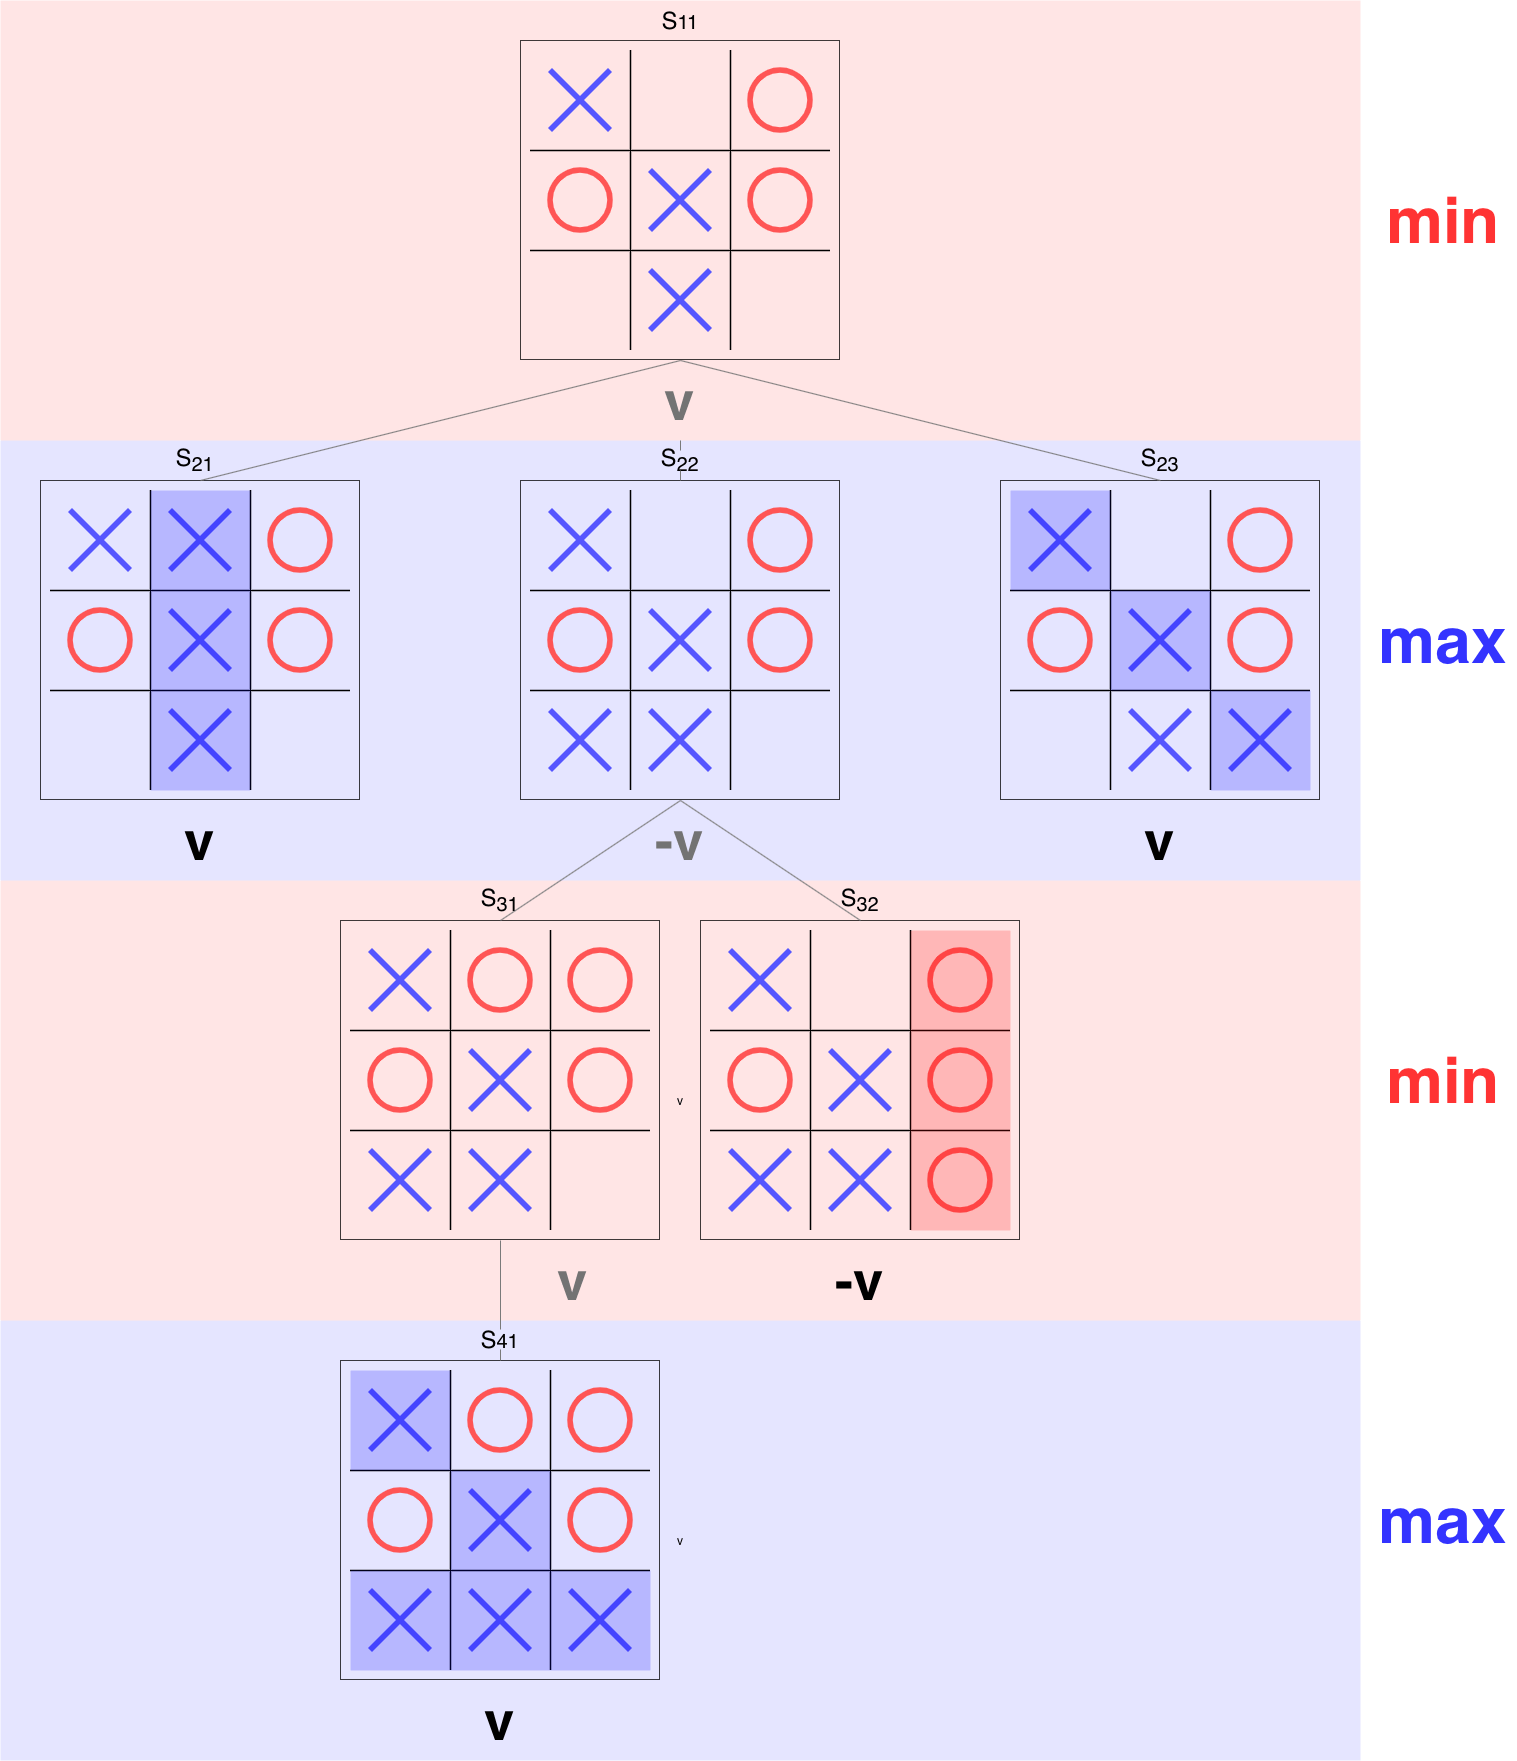
\includegraphics[width=0.8\textwidth]{images/minmax-tree.png}
    \caption{Rozhodovací strom algoritmu Minimax}
\end{figure}\label{figure:minimax-tree}

Algoritmus minimax patrí medzi \emph{exaktné algoritmy}, čo znamená, že pri hľadaní nájde najlepšie (optimálne)
riešenie, no prehľadáva všetky možné riešenia (celý vyhľadávací priestor).
Vo všeobecnosti pre neprázdne hracie pole o veľkosti $r$ v $d$-rozmernom hracom priestore s $o$ obsadenými políčkami je
možné veľkosť celého vyhľadávacieho priestoru vypočítať ako
\begin{equation}
    C(r, d, o) = (r^d - o) * (r^d - o - 1) * (r^d - o - 2) \dots 1 = \prod_{i = 1}^{r^d - o}{(r^d - o - i + 1)}
\end{equation}
Pre prázdne hracie pole (teda, kde $o = 0$) platí
\begin{equation}
    C(r, d, 0) = (r^d) * (r^d - 1) * (r^d - 2) \dots 1 = \prod_{i = 1}^{r^d}{(r^d - i + 1)}
\end{equation}

Ak algoritmus vychádza z prázdneho poľa o veľkosti $3 \times 3$ ($r = 3$, $d = 2$) je veľkosť vyhľadávacieho priestoru
$\prod_{i = 1}^{9}{(10 - i)} =$ \textbf{362 880}.
Na preskúmanie takéhoto počtu je možné použiť aj komerčnú výpočtovú techniku pričom výsledok bude známy v čase menšom
ako jedna minúta, no pri veľkosti $4 \times 4$ (teda $r = 4$, $d = 2$) je $C(4, 2, 0) \approx 2*10^{13}$ a čas
prehľadania priestoru sa (za predpokladu, že preskúmanie 1 možnosti trvá 1 milisekundu) zvýši na
\emph{$\approx 663$ rokov}.
Pre trojrozmernú plochu s rozmerom $3$ ($r = 3$, $d = 3$) je $C(3, 3, 0) \approx 1.08 * 10^{28}$, čo s rovnakým časovým
predpokladom znamená, že takýto výpočet by sa skončil po $\approx 3*10^{17}$ rokoch (pre predstavu: vek vesmíru sa
odhaduje na $\approx 14$ mld. $\approx 14 * 10^9$ rokov).

\subsection{Umelá neurónová sieť}\label{subsec:algo-ann}

Z vyššie uvedeného vyplýva, že exaktné riešenie pre väčšie rozmery plochy nie je možné použiť, teda je nutné použiť
algoritmy, ktoré nenájdu najlepšie riešenie v rámci celého vyhľadávacieho priestoru (optimálne), no vedia nájsť
najlepšie riešenie v rámci obmedzeného vyhľadávacieho priestoru (suboptimálne).
Jednou z týchto heuristických metód je \emph{umelá neurónová sieť} angl. artificial neural network
(často označovaná ako ANN).

Matematické základy pre tento algoritmus boli vytvorené už v polovici 20. storočia a sú založené na modeli
biologických neurónových sietí, z čoho vychádza aj názov a terminológia.\cite{algo_ann_history}
Sieť pozostáva z \textbf{vrstiev}, ktoré sú tvorené \textbf{neurónmi}.
Medzi jednotlivými neurónmi sú prepojenia nazývané tiež \textbf{synapsy}.\cite{algo_ann_terminology}
Umelú neurónovú sieť je možné reprezentovať ohodnoteným \hyperref[figure:general-ann]{grafom}, kde vrcholy reprezentujú
neuróny a hrany synaptické spojenia.
Graf môže vyzerať nasledovne:
\begin{figure}[H]
    \centering
    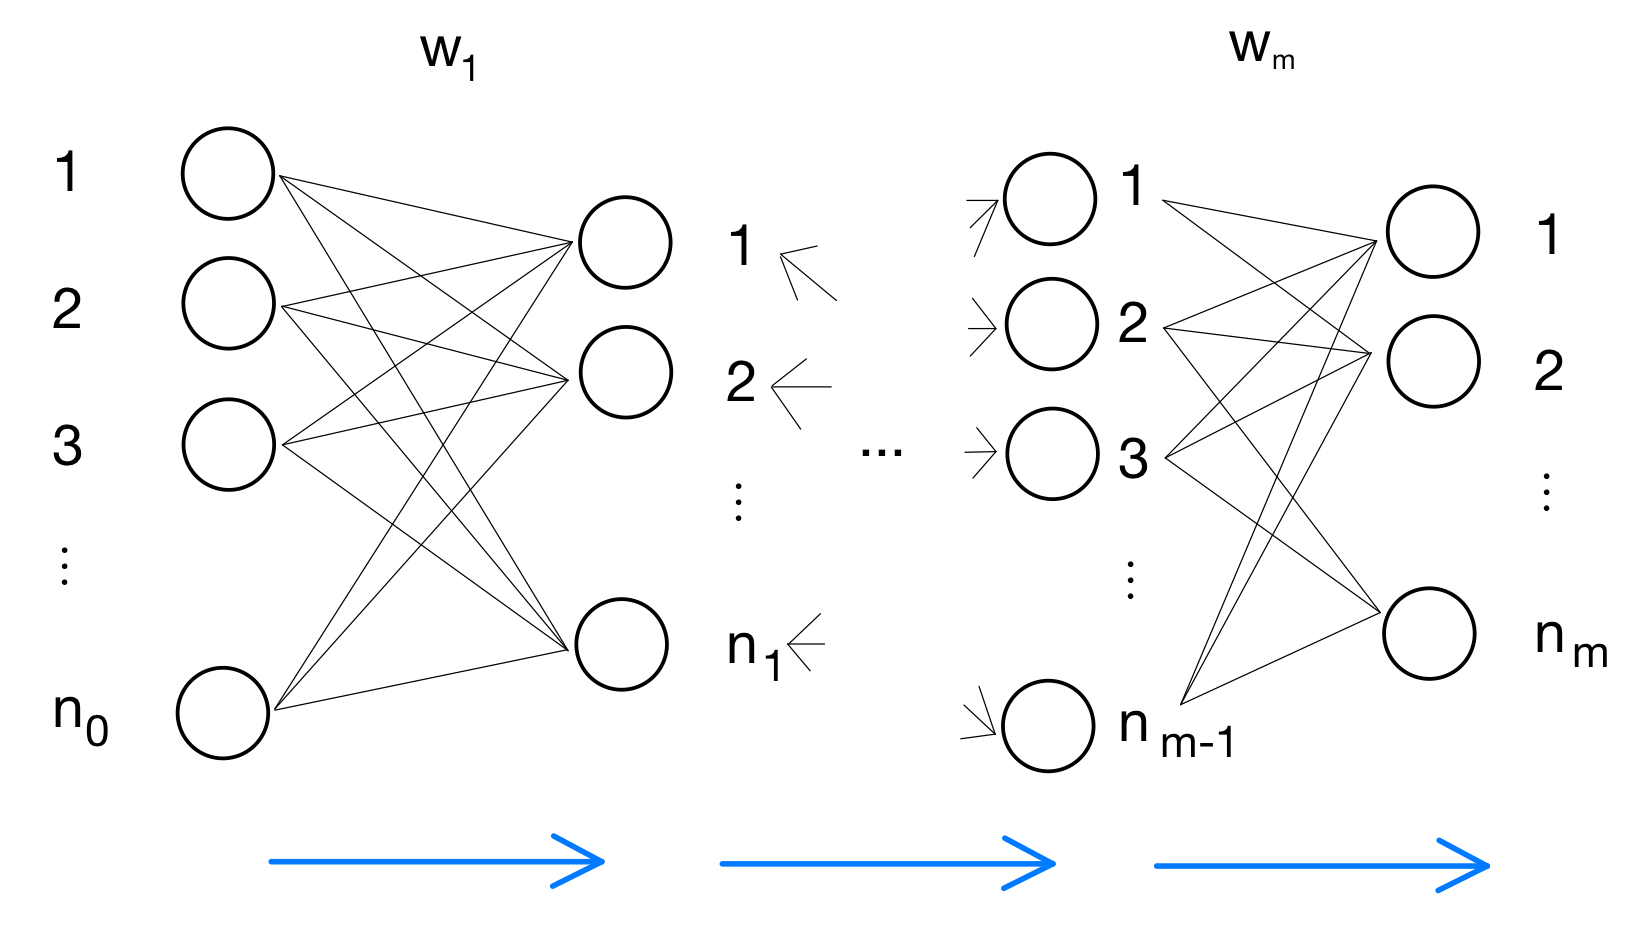
\includegraphics[width=0.5\textwidth]{images/general-ann.jpg}
    \caption{Všeobecná dopredná umelá neurónová sieť}
\end{figure}\label{figure:general-ann}
Nech $m$ je počet vrstiev v umelej neurónovej sieti a $n_i$ pre $i = 0 \dots m$ je počet neurónov vo vrstve $i$.
Existuje mnoho typov umelých neurónových sietí, no všeobecne sa ako ANN označuje dopredná umelá neurónová sieť.
V doprednej ANN existujú synapsy (spojenia) len medzi vrstvami $i$ a $i + 1$ pre $i = 0 \dots m - 1$, tzn. spojenia
existujú len medzi za sebou idúcimi vrstvami smerom od vstupnej ($i=0$) k výstupnej ($i=m$) vrstve.

Každému neurónu je priradená aktivačná funkcia.
Z biologického hľadiska vyjadruje akčný potenciál bunky a teda prenos informácie cez synaptické prepojenie.
V rámci umelých neurónových sietí aktivačná funkcia vyjadruje to isté: je to binárna funkcia a neurón sa aktivuje
ak na výstupe z tejto funkcie je 1.
Aktivačná funkcia závisí od vstupov predchádzajúcich neurónov.
Nech $N_{ij}$ pre $i = 1 \dots m-1$, $j = 1 \dots n_i$ je $j$-ty neurón v $i$-tej vrstve.
Na vstup do tohto neurónu sa z predchádzajúcej vrstvy prenesú informácie vo vektore $\pmb{x_{ij}}$.
$\forall h \in \pmb{x_{ij}} \colon h \in \{0, 1\}$.
Pre všetky synaptické spojenia existujú tzv. \emph{váhy}, ktoré zosilňujú (resp. zoslabujú) účinok signálu z
predchádzajúcich neurónov.
Nech $w_{ijk}$ pre $i=1 \dots m$, $k=1 \dots n_{i-1}$, $j=1 \dots n_i$ je váha pre synaptické spojenie vedúce z
neurónu $k$ vo vrstve $i-1$ k neurónu $j$ vo vrstve $i$ resp.
nech vektor $\pmb{w_{ij}}$ je vektor váh definovaných pre neurón $N_{ij}$ a nech
\begin{equation}
    z = \sum_{k=1}^{|\pmb{w_{ij}}|=|\pmb{x_{ij}}|}{w_{ijk} * x_{ijk}}-\theta
\end{equation}
kde $\theta$ je tiež označovaná ako prahová hodnota (angl. threshold).
\hyperref[figure:activation-functions]{Aktivačná funkcia} sa označuje ako $\phi(z)$.
Medzi bežne používané aktivačné funkcie patrí napríklad:
\linebreak
\textbf{SoftMax} (táto aktivačná funkcia sa využíva pri kategorizácii)\cite{algo_ann_activation_softmax}
\begin{equation}
    \phi(\mathbf{z})_i = \frac{e^{z_i}}{\sum_{j=1}^{|z|}{e^{z_j}}}
\end{equation}
\textbf{Sigmoid}\cite{algo_ann_activation_sigmoid}
\begin{equation}
    \phi(z) = \frac{1}{1+e^{-z}}
\end{equation}
\textbf{Hyperbolická funkcia}\cite{algo_ann_activation_hyperbolic}
\begin{equation}
    \phi(z) = tanh(z)
\end{equation}
\textbf{ReLu}\cite{algo_ann_activation_relu}
\begin{equation}
    \phi(z) = \max\{0, x\}
\end{equation}

Priebehy niektorých týchto funkcií sú zobrazené na grafe.
\begin{figure}[H]
    \centering
    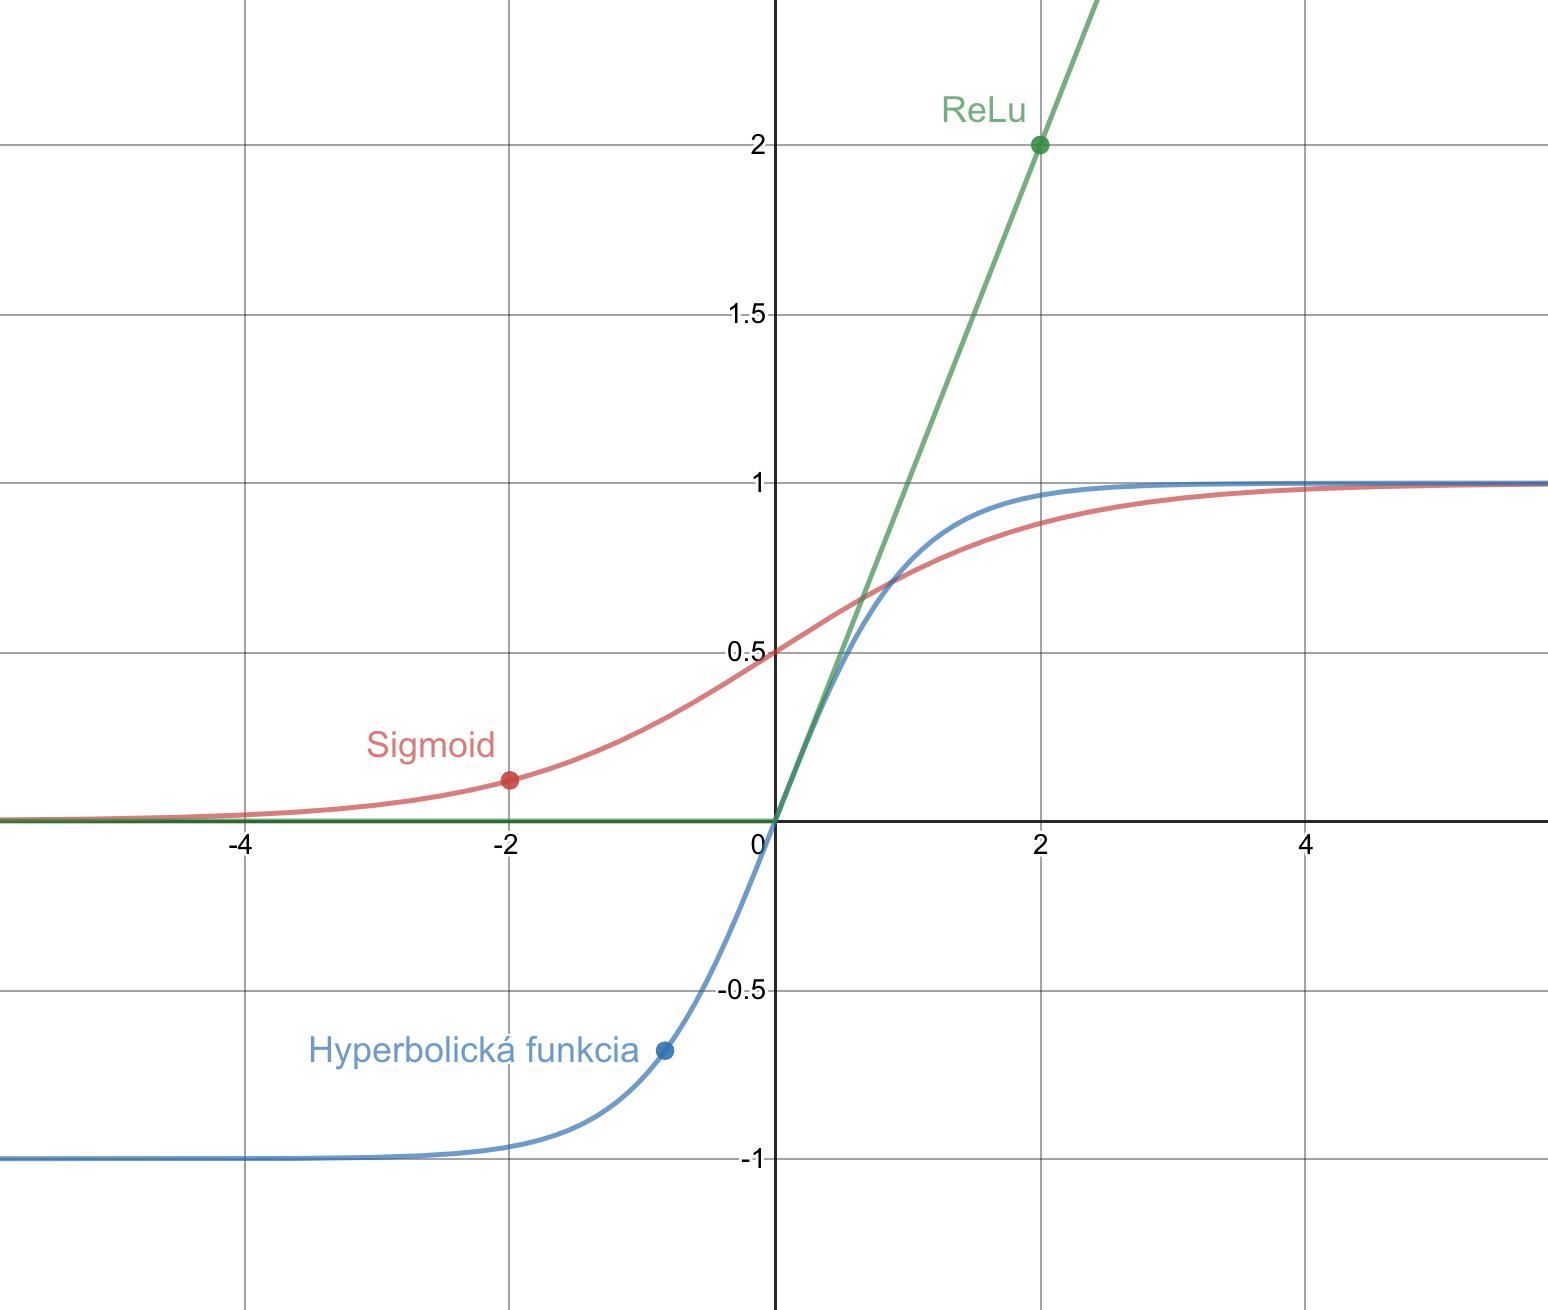
\includegraphics[width=0.8\textwidth]{images/activation-functions.png}
    \caption{Priebehy aktivačných funkcií}
\end{figure}\label{figure:activation-functions}

Pri vytváraní umelej neurónovej siete je potrebné dbať na jej správnu štruktúru a nastavenie váh.
Váhy sa dajú nastaviť tzv. učením siete.
Učenie prebieha v 2 fázach: trénovanie a testovanie siete.
V prvej fáze sa sieť naplní \emph{existujúcimi} vstupmi a výstupmi, aby vedela odhadnúť vzťah medzi nimi.
Existuje mnoho tréningových metód, no v tejto práci sú popísané 2:
\begin{itemize}
    \item algoritmus založený na delta prístupe\cite{algo_ann_delta_rule}
    \item algoritmus založený na spätnom šírení\cite{algo_ann_backpropagation}
\end{itemize}
Pri oboch prístupoch je nutné definovať tzv. trénovaciu ($T_r$) a testovaciu množinu ($T_t$).
Trénovacia množina slúži na prvotné nastavenie parametrov (váh).
Využíva sa vo fáze trénovania.
Natrénovaná sieť sa v druhej fáze otestuje pomocou testovacej množiny.

Pri \textbf{algoritme založenom na delta prístupe} (ďalej len "delta algoritmus") sa pracuje len s dvojvrstvovou
umelou neurónovou sieťou (resp. s vrstvou, ktorá ma len jednu sadu synaptických prepojení).
Princíp spočíva v postupnom vyhodnocovaní rozdielu medzi výstupom z umelej neurónovej siete pri určitom vstupe
(reálny výstup) a správnym výstupom (očakávaný výstup).
Parametre ANN sú upravované v závislosti od tohto rozdielu.
Nech $\gamma \in (0, \infty)$ je učiaci parameter, $\epsilon$ je maximálny akceptovateľný rozdiel v hodnotách reálneho
a očakávaného výstupu a $s$ je počet za sebou idúcich rozdielov výstupov (rozdiel nemusí byť vyhodnocovaný len
prostredníctvom absolútnej hodnoty, často sa využíva aj druhá mocnina rozdielu), ktoré sa nachádzali v rámci $\epsilon$.
Ďalej nech $|T_r|$ je veľkosť trénovacej množiny (teda počet vzoriek), $\mathbf{X_i}$ pre $i=1 \dots |T_r|$ je vzorka
z trénovacej množiny, ktorej je pridelený očakávaný výstup $y_i$ pre $i=1 \dots |T_r|$ a nech $y(\mathbf{X_i})$ je reálny
výstup siete ako odpoveď na vstup $\mathbf{X_i}$.
Algoritmus prebieha nasledovne:\cite{algo_ann_delta_rule}
\begin{enumerate}
    \item Inicializácia počiatočných váh $\pmb{w_1}$, prahovej hodnoty $\theta$ a parametrov $\gamma$, $\epsilon$ a $s$.
    \item pre $i = 1 \dots |T_r|$:
    \begin{enumerate}
        \item ak $(y_i-y(\mathbf{X_i}))^2>\epsilon$ \\
                $\Delta{w_j} = \gamma * (y_i-y(\mathbf{X_i}))_j$ \\
                $\pmb{w_{1j}}=\pmb{w_{1j}} + \Delta{w_j} * X_{ij}$ \\
                $\theta=\theta + \Delta{w_j}$
        \item ak prebehlo $s$ za sebou idúcich rozdielov výstupov, ktoré sa nachádzali v rámci $\epsilon$, tak koniec
    \end{enumerate}
\end{enumerate}
Zmena váh o vektor $y_i-y(\mathbf{X_i})$ je celkom intuitívna, no je možné si ukázať, že to funguje aj matematicky.
Nech $\pmb{\omega_0}$ je východiskový bod pre váhy a nech $f(\pmb{x})$ je funkcia vyjadrujúca mieru chyby v sieti,
ktorú je potreba minimalizovať.
K bodu $\pmb{\omega_1}$ je možné sa z východiskového bodu posunúť v jednotkovom smere $\pmb{d}$ ($|\pmb{d}|=1$) o krok
dĺžky $\alpha$, tzn.
\begin{equation}
    \pmb{\omega_1} = \pmb{\omega_0} + \alpha\pmb{d}
\end{equation}
Tu sa naskytá otázka ako zvoliť veľkosť kroku $\alpha$, tak aby $f(\pmb{\omega_1}) < f(\pmb{\omega_0})$.
\textbf{Derivácia} funkcie vyjadruje zmenu akejkoľvek funkcie $f(x)$ v pomere s čo najmenšou zmenou parametrov tejto
funkcie, teda
\begin{equation}
    \lim_{\alpha\to0}\frac{|f(x + \alpha) - f(x)|}{\alpha}
\end{equation}
kde $\alpha$ vyjadruje zmenu parametrov.
Keďže $f(\omega_1)=f(\omega_0+\alpha\pmb{d})$ je možné tento princíp použiť na výpočet kroku $\alpha$.
\begin{equation}
    \frac{d}{d\alpha}f(\pmb{\omega_0}+\alpha\pmb{d}) = \
    \sum_{\forall i}{\frac{d f(\omega_{0_i} + \alpha{d_i})}{d \omega_{0_i} + \alpha{d_i}}}*\frac{d}{d\alpha}\omega_0+\alpha\pmb{d} = \
    \sum_{\forall i}{\frac{d f(\omega_{0_i} + \alpha{d_i})}{d \omega_{0_i} + \alpha{d_i}}}*\pmb{d} = \
    \pmb{f'}(\pmb{\omega_0}+\alpha\pmb{d})*\pmb{d}
\end{equation}
a keďže $\alpha\to0$, potom výraz je možné upraviť na
\begin{equation}
    \pmb{f'}(\pmb{\omega_0})*\pmb{d}
\end{equation}
a je to zároveň \emph{gradient} funkcie $\pmb{f}$ v bode $\pmb{\omega_0}$.
Pre skalárny súčet dvoch vektorov $\pmb{a}$ a $\pmb{b}$ platí $\pmb{a} * \pmb{b} = |\pmb{a}| * |\pmb{b}| * \cos(\beta)$, kde $\beta$
je uhol, ktorý tieto vektory zvierajú.
Keďže $\pmb{f'}(\pmb{\omega_0})$ a $\pmb{d}$ sú vektory a $|\pmb{d}|=1$ platí
\begin{equation}
    |\pmb{f'}(\pmb{\omega_0})| * \cos(\beta)
\end{equation}
Pretože $|\pmb{f'}(\pmb{\omega_0})|$ je konštanta, je potrebné vhodne zvoliť $\cos(\beta)$ tak, aby celý výraz bol čo
najmenší.
\begin{equation}
    H(\cos(\beta)) = <-1,1> \implies \cos(\beta) = -1 \iff \beta = -180\degree = -\pi
\end{equation}
Z toho vyplýva, že smer najlepšieho poklesu je opačný ku gradientu funkcie (teda $-\pmb{f'}(\pmb{\omega_0})$).
V prípade delta algoritmu je minimalizovaná funkcia rozdielu reálneho a očakávaného výstupu
\begin{equation}
    f(\pmb{\omega})=(y_i-y(\mathbf{X_i}))^2=(y_i-\phi(\sum_{\forall j}{\omega_j X_{ij}-\theta}))^2
\end{equation}
\begin{equation}
    \frac{\partial}{\partial \omega_k}f(\pmb{\omega})=2*(y_i-\phi(\sum_{\forall j}{\omega_j X_{ij}-\theta}))*(-\phi'(\sum_{\forall j}{\omega_j X_{ij}-\theta}))*X_{ik}
\end{equation}
\begin{equation}
    \frac{\partial}{\partial \omega_k}f(\pmb{\omega})=-(y_i-y(\mathbf{X_i}))*X_{ik}*(2(-\phi'(\sum_{\forall j}{\omega_j X_{ij}-\theta})))
\end{equation}
Posledný činiteľ je kladný (tzn. nezmení znamienko výrazu - derivácia kladnej funkcie) a teda smer najväčšieho poklesu
je
\begin{equation}
    \pmb{d}=(y_i-y(\mathbf{X_i}))*X_{ik}
\end{equation}
Z vyššie uvedeného vyplývajú isté vlastnosti: keďže $\phi$ je aktivačná funkcia, tak pre správne fungovanie delta
algoritmu je nutné aby bola \emph{derivovateľná}.

\textbf{Algoritmus založený na spätnom šírení} (angl. a ďalej len "backpropagation algoritmus") je zovšeobecnenie delta
algoritmu pre viacvrstvové siete.
Funguje na rovnakom princípe, ktorý sa postupne opakuje smerom od výstupnej vrstvy k vstupnej.

Vyššie popísaná metóda optimalizácie sa nazýva aj gradientová metóda najväčšieho poklesu.
Pri tejto metóde existuje niekoľko vylepšení, resp. alternatív, ktoré sa týkajú najmä parametrov, ktoré sa môžu meniť
aj dynamicky, väčšinou sú tieto metódy koncepčne veľmi podobné.
Riešenie potom rýchlejšie konverguje k optimálnym hodnotám.
Nižšie sú popísané najpoužívanejšie alternatívy.
\paragraph{RMSProp}\cite{algo_ann_optimizer_rmsprop}
Z anglického \enquote{\textbf{R}oot \textbf{m}ean \textbf{s}quare \textbf{prop}agation}.
Algoritmus vychádza z gradientovej metódy, no upravuje hodnotu, ktorá sa pripočítava k váham, aby sa zabránilo oscilácii
metódy okolo optimálnej hodnoty.
RMSProp upravuje zmenu váh nasledovne:
\begin{equation}
    v_j=pv_j+(1-p)(y_i-y(\mathbf{X_i}))_j^2
\end{equation}
\begin{equation}
    \Delta{w_j}=-\frac{\eta}{\sqrt{v_j+\epsilon}}(y_i-y(\mathbf{X_i}))_j
\end{equation}
Kde $\eta$ je počiatočný učiaci parameter.
$p \in <0,1>$ zvyčajne $p=0.9$, $\epsilon$ je použitý len na to, aby sa predišlo deleniu nulou a zvyčajne
$\epsilon = 10^{-10} = 1e-10$ a $v_j$ je priemer umocnených gradientov.
Hodnota $\Delta{w_j}$ je potom pripočítaná k váham.
\paragraph{Adam}\cite{algo_ann_optimizer_adam}
Odvodené z anglického \enquote{\textbf{Ada}ptive \textbf{m}oment optimization}.
Algoritmus vychádza z gradientovej metódy, no upravuje hodnotu, ktorá sa pripočítava k váham, aby sa zabránilo oscilácii
metódy okolo optimálnej hodnoty.
Adam upravuje zmenu váh nasledovne:
\begin{equation}
    v_j=\beta_1{v_j}-(1-\beta_1)(y_i-y(\mathbf{X_i}))_j
\end{equation}
\begin{equation}
    s_j=\beta_2{s_j}-(1-\beta_2)(y_i-y(\mathbf{X_i}))_j^2
\end{equation}
\begin{equation}
    \Delta{w_j}=-\eta\frac{v_j}{\sqrt{s_j+\epsilon}}(y_i-y(\mathbf{X_i}))_j
\end{equation}
Kde $\eta$ je počiatočný učiaci parameter.
$p \in <0,1>$ zvyčajne $p=0.9$, $\epsilon$ je použitý len na to, aby sa predišlo deleniu nulou a zvyčajne
$\epsilon = 10^{-10} = 1e-10$, $v_j$ je priemer gradientov a $s_j$ je priemer umocnených gradientov.
Hodnota $\Delta{w_j}$ je potom pripočítaná k váham.

Pri návrhu je možné určiť aj účelovú funkciu optimalizácie tréningu a teda spôsob, akým tréningový proces vyhodnocuje
správnosť, resp. nesprávnosť výstupu pri danom vstupe.
Nech $E(w, y, \hat{y})$ je chyba výsledku pri parametri $w$ a výstupe $\hat{y}$ s očakávaným výstupom $y$
a $F(E(w, y, \hat{y}))$ je účelová funkcia optimalizačného procesu.
\paragraph{Priemerná štvorcová chyba}\cite{algo_ann_mse}
Anglicky \emph{mean squared error} (skr. MSE).
\begin{equation}
    F(E(w, y, \hat{y}))=E(w, y, \hat{y})^2
\end{equation}
\paragraph{Priemerná absolútna chyba}\cite{algo_ann_mae}
Anglicky \emph{mean absolute error}.
\begin{equation}
    F(E(w, y, \hat{y}))=|E(w, y, \hat{y})|
\end{equation}
\paragraph{Kategorická krížová entropia}\cite{algo_ann_categorical_crossentropy}
Anglicky \emph{categorical crossentropy}.
Táto účelová funkcia vyžaduje, aby vstupy boli kategorizované, čoho dôsledkom je aj to, že táto účelová funkcia sa
využíva pri kategorizácii vstupov.
\begin{equation}
    E(w, y, \hat{y})=y*\log(\hat{y})
\end{equation}

Navrhnutie štruktúry umelej neurónovej siete je jeden z najťažších problémov pri vytváraní riešenia problému.
Neexistuje jednoznačná a univerzálna cesta vytvorenia, ktorá by platila pre všetky problémy.
Pre jednoduché problémy je možné použiť matematické metódy pre vytvorenie umelej neurónovej siete, no pre tie väčšie
sa ANN vytvárajú skôr využitím intuície architekta siete.

\subsubsection{Umelá neurónová sieť pre hru}

Keďže váhy je možné upraviť pomocou trénovania ostáva ešte určiť štruktúru umelej neurónovej siete.
ANN by mala spĺňať tieto vlastnosti:
\begin{itemize}
    \item na vstupe má byť aktuálny stav hry
    \item na výstupe má byť informácia o tom, ktoré pole je pre aktuálneho hráča najlepšie pre ďalší krok
\end{itemize}

Stav hry je reprezentovaný vektorom $s_i$ pre $i=1 \dots r^d$, kde každých $r$ prvkov reprezentuje riadok hracej plochy,
resp. hracieho priestoru.
Napríklad pre rozmer $3 \times 3$ má vektor $s$ dĺžku 9 ($r^d=3^2$), prvky 1--3 reprezentujú prvý riadok, prvky
4--6 reprezentujú druhý riadok a prvky 7--9 reprezentujú posledný riadok.
Neurónová sieť pozostáva z 3 vrstiev (vstupná, skrytá, výstupná).
Nech $x_i$ pre $i=1 \dots 3r^d$ je neurón vo vstupnej vrstve.
Za vstup do neurónovej siete je považovaný vektor hodnôt $x_1$ až $x_{3r^d}$, kde
\begin{equation}
    x_i=
    \begin{cases}
        1 & \text{ak }s_i\text{ je prázdne a } i \in \langle 1, r^d \rangle \\
        1 & \text{ak }s_{i-r^d}\text{ je cieľový hráč a } i \in \langle r^d+1, 2r^d \rangle \\
        1 & \text{ak }s_{i-2r^d}\text{ je oponent a } i \in \langle 2r^d+1, 3r^d \rangle \\
        0 & \text{inak}
    \end{cases}
    \quad
    \text{pre }i=1 \dots 3r^d
\end{equation}
Nech $y_j$ pre $j=1 \dots r^d$ je neurón v skrytej vrstve.
Táto vrstva zabezpečuje reprezentáciu stavu hry, na základe ktorej sa nastavujú váhy pre jednotlivé hodnoty políčok
hracej plochy.
Tieto váhy je možné označiť $w_{ij}$ pre $i=1 \dots 3r^d$, $j=1 \dots r^d$, kde index $ij$ vyjadruje váhu hodnoty
$x_i$ vstupujúcu do neurónu $y_j$.
Zo vstupnej vrstvy do skrytej vrstvy sa teda prenesú hodnoty
\begin{equation}
    \sum_{i=1}^{3r^d} w_{ij}x_{ij} \quad \text{pre } j=1 \dots r^d
\end{equation}
Posledná (skrytá) vrstva má len jeden neurón $z$, ktorý vyjadruje index $i$ vo vektore $s_i$ pre najlepší možný ťah
hráča.
Váhy zo skrytej vrstvy vstupujúce do poslednej vrstvy je možné označiť $v_j$.
Zo skrytej vrstvy do výstupnej vrstvy sa prenesú hodnoty
\begin{equation}
    \sum_{j=1}^{r^d} v_{j}y_{j}
\end{equation}
Neurónová sieť vyzerá nasledovne:

\begin{figure}[H]
    \centering
    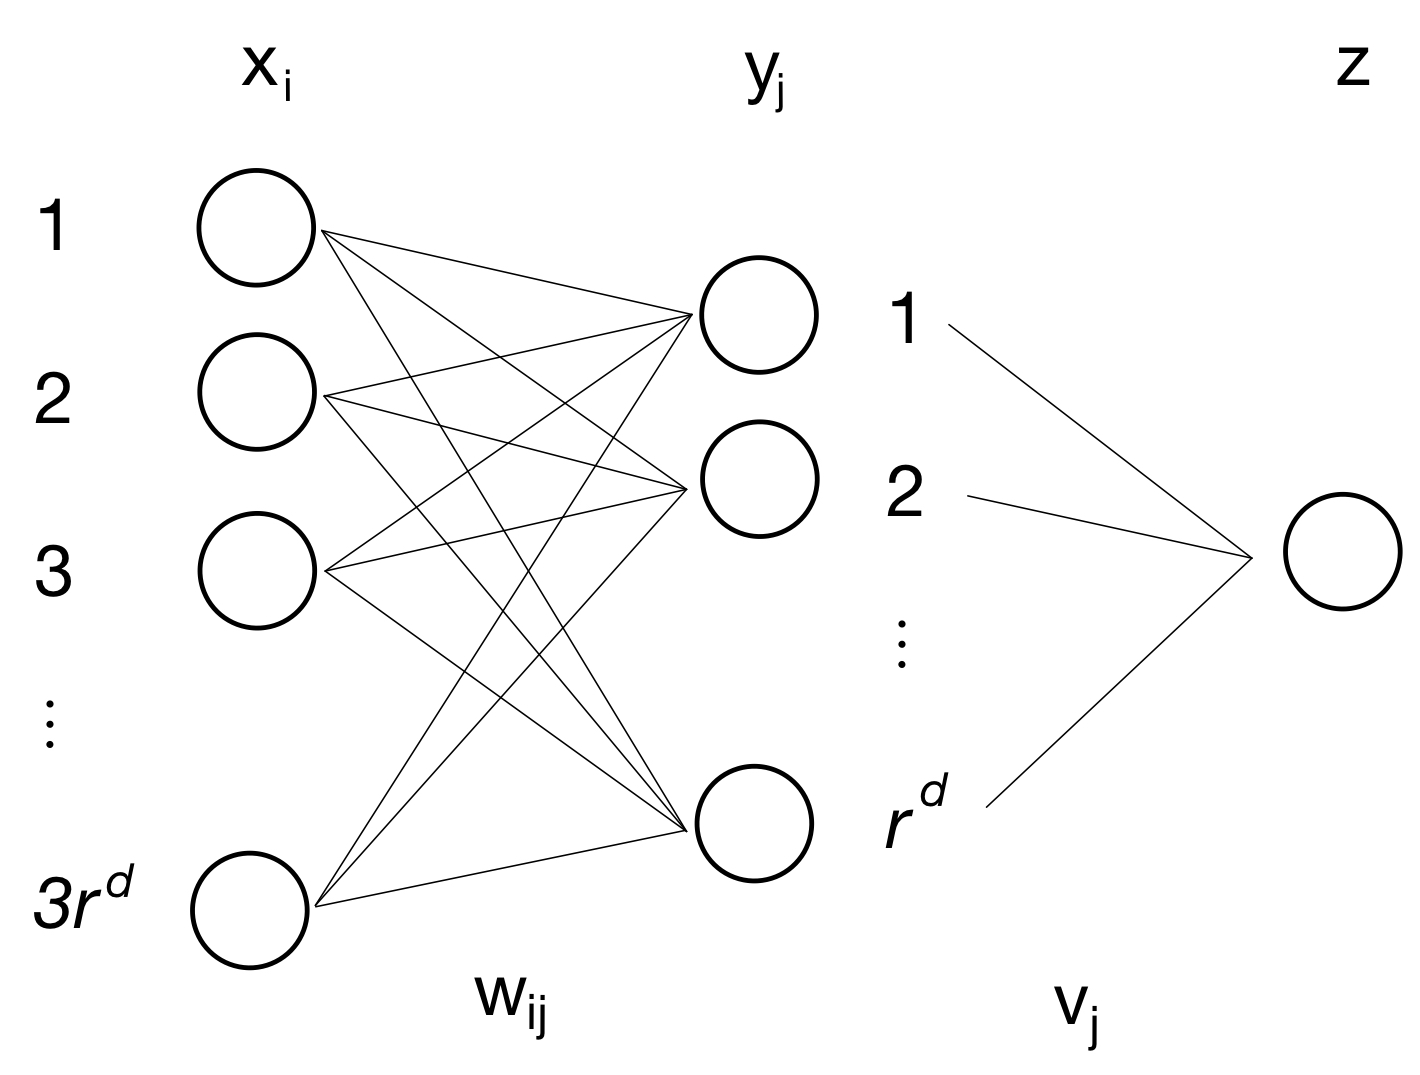
\includegraphics[width=0.5\textwidth]{images/ann.jpg}
    \caption{Návrh neurónovej siete}
\end{figure}
Implementácia tejto neurónovej siete je bližšie popísaná v \autoref{subsec:dev-tools-for-ai}.

Pre potreby natrénovania umelých neurónových sietí boli použité simulácie náhodných hier.
Simulácie pozostávali z náhodného výberu políčok pre každého hráča.
Náhodný výber bol navyše zlepšený predpokladom, že hráči sa počas hry (najmä na plochách väčších rozmerov) snažia
väčšinou znemožniť protihráčovi jeho výhru výberom políčok, ktoré sú blízko jeho predchádzajúcemu ťahu
(resp. predchádzajúcim ťahom).
Keďže piškvorky sú hra, ktorá sa hrá na pravouhlej ploche (resp. pravouhlom priestore) bolo možné pri výpočte
pravdepodobnosti výberu prvku použiť Manhattanskú vzdialenosť.
Nech pre $d=3$ $c_i(b)$, $c_j(b)$, $c_k(b)$ sú súradnice ($i$ a $j$) políčka, ktoré je najbližšie k políčku $b_{ijk}$ a
nech
\begin{equation}
    e(b_{ijk}) =
    \begin{cases}
        1 & \text{ak políčko }ijk\text{ je prázdne} \\
        0 & \text{inak}
    \end{cases}
\end{equation}
potom pravdepodobnosť výberu políčka $ijk$ je
\begin{equation}
    p(b_{ijk}) = \frac{|c_i(b) - i| + |c_j(b) - j| + |c_k(b) - k|}{\sum_{m=1}^r\sum_{n=1}^r\sum_{o=1}^r e(b_{mno})}
\end{equation}
Pre $d=2$ (teda pre hru na ploche) platia rovnaké pravidlá, pričom $k=1$ (resp. $o=1$) vo všetkých prípadoch.

\subsection{Zisťovanie víťaza}\label{subsec:checking-winner}

Už kontrola víťaza pre plochu (2D priestor) s pevne danými rozmermi a pevne danou hodnotou počtu znakov potrebných pre
výhru (často zhodnou s rozmerom) je relatívne komplexná úloha.
Ak sú použité sofistikovanejšie prostriedky než fixný prístup k prvkom poľa prostredníctvom číselných indexov, tak pre
rozmer $r \times r$, kde $r = w$ má tento problém nasledovné riešenie:
\begin{lstlisting}[
  mathescape,
  columns=fullflexible,
  basicstyle=\fontfamily{lmvtt}\selectfont,
]
pre $i=1\dots{r}$:
    ak $b_{i0}$ je prázdne
    inak:
        $z = b_{i0}$
        pre $j=1\dots{r}$:
            ak $b_{ij} \neq z$:
                prejdi na ďalší riadok
        víťaz je $z$
pre $j=1\dots{r}$:
    ak $b_{0j}$
    inak:
        $z = b_{0j}$
        pre $i=1\dots{r}$:
            ak $b_{ij} \neq z$:
                prejdi na ďalší stĺpec
        víťaz je $z$
ak $b_{00}$ nie je prázdny znak
    $z = b_{00}$
    pre $i=1\dots{r}$:
        ak $b_{ii} \neq z$, koniec cyklu
    víťaz je $z$
ak $b_{0,r-i}$ nie je prázdny znak
    $z = b_{0,r-i}$
    pre $i=1\dots{r}$:
        ak $b_{i,r-i} \neq z$, koniec cyklu
    víťaz je $z$
ak žiadny z predošlých cyklov nevyhodnotí víťaza a
neexistuje žiaden možný ťah pre hráča, nastala remíza
\end{lstlisting}
Prvá a druhá časť skúmajú potenciálnych víťazov v riadku a stĺpci, druhá časť skúma výsledky diagonálne.
Keďže $r = w$ stačí preskúmať hlavnú a vedľajšiu diagonálu, pretože tie sú jediné, ktoré môžu obsahovať $w$ znakov.
Zložitosť tohto algoritmu je exponenciálna:
\begin{equation}
    \mathcal{O}(r.r + r.r + 2r + 2r) \sim \mathcal{O}(2r^2 + 4r) \sim \mathcal{O}(r^2)
\end{equation}

Nech $R$ je množina potenciálnych víťazných množín $M$ ($|M|=r$).
Algoritmus je možné prepísať nasledovne:
\begin{lstlisting}[
  mathescape,
  columns=fullflexible,
  basicstyle=\fontfamily{lmvtt}\selectfont,
]
$R=\{\}$
$M_h=\{\}$
$M_v=\{\}$
pre $i=1\dots{r}$:
    $M_r=\{b_{ij}|j=1 \dots r\}$
    pridanie $M_r$ do $R$
    $M_s=\{b_{ji}|j=1 \dots r\}$
    pridanie $M_s$ do $R$
    pridanie $b_{ii}$ do $M_h$
    pridanie $b_{i,r-i}$ do $M_v$

pridanie $M_h$ do $R$
pridanie $M_v$ do $R$

pre $k=1\dots{|R|}$:
    $z$ = $k$-ty prvok z $R$
    pre $i=1\dots{r}$:
        ak $z_0 = z_i$, potom $z_0$ je víťaz
ak predošlý cyklus nevyhodnotí víťaza a
neexistuje žiaden možný ťah pre hráča, nastala remíza
\end{lstlisting}
Algoritmus najskôr vytvorí množinu $R$ z každého stĺpca a riadku ($M_r$ a $M_s$) a postupne plní množiny hlavnej a
vedľajšej diagonály ($M_h$ a $M_s$).
Za predpokladu, že $R$ je reprezentovaná štruktúrou, kde zložitosť vloženia je $\mathcal{O}(1)$ a
$|R| = r + r + 2 = 2r + 2$, potom celková zložitosť je znova exponenciálna, no algoritmus je omnoho kratší
\begin{equation}
    \mathcal{O}(r.2r + r.|R|) \sim \mathcal{O}(r.2r + r.(2r + 2)) \sim \mathcal{O}(2r^2 + 2r^2 + 2r) \sim \mathcal{O}(4r^2 + 2r) \sim \mathcal{O}(r^2)
\end{equation}

Takýto algoritmus je celkom jednoduchý a má prijateľnú (exponenciálnu) zložitosť vzhľadom na rozmer hracej plochy.
V prípade, že $r \neq w$, je nutné algoritmus rozšíriť.
Jeden zo spôsobov je taký, že vždy sa kontroluje iba plocha o veľkosti $w \itmes w$ (vyššie popísaným algoritmom) s
tým, že kontrolovaná plocha $W$ začína na počiatočných súradniciach $[x,y]=[1,1]$ a postupne sa súradnice zvyšujú o 1
tak, aby boli skontrolované všetky kombinácie počiatočných súradníc.
Počiatočné súradnice $x$ a $y$ nadobúdajú hodnoty z $C = \{1, 2, \dots, r - w\}$.
Algoritmus je možné upraviť nasledovne:
\begin{lstlisting}[
  mathescape,
  columns=fullflexible,
  basicstyle=\fontfamily{lmvtt}\selectfont,
]
Nech $skontroluj(x, y)$:
    $R=\{\}$
    $M_h=\{\}$
    $M_v=\{\}$
    pre $i=x\dots{x + w}$:
        $M_r=\{b_{ij}|j=y \dots y + w\}$
        pridanie $M_r$ do $R$
        $M_s=\{b_{ji}|j=y \dots y + w\}$
        pridanie $M_s$ do $R$
        pridanie $b_{ii}$ do $M_h$
        pridanie $b_{i,r-i}$ do $M_v$

    pridanie $M_h$ do $R$
    pridanie $M_v$ do $R$

    pre $k=1\dots{|R|}$:
        $z$ = $k$-ty prvok z $R$
        pre $i=1\dots{w}$:
            ak $z_0 = z_i$, potom $z_0$ je víťaz
    ak predošlý cyklus nevyhodnotí víťaza tak:
        ak $[x + 1, y]$ nebolo skontrolované $skontroluj(x + 1, y)$
        ak $[x, y + 1]$ nebolo skontrolované $skontroluj(x, y + 1)$
        ak $[x + 1, y + 1]$ nebolo skontrolované $skontroluj(x + 1, y + 1)$

$skontroluj(0, 0)$
\end{lstlisting}
Keďže procedúra $skontroluj$ je volaná vnútri jej definície, je jasné, že táto procedúra je \emph{rekurzívna}.
Nech $c = |C| = r - w$, potom počet volaní $skontroluj$ je $c$ a ak zložitosť procedúry $skontroluj(x, y)$ je
$\mathcal{O}(4r^2 + 2r)$, potom celková zložitosť je
\begin{equation}
    \mathcal{O}((4r^2 + 2r).c^2) \sim \mathcal{O}(4r^2c^2 + 2rc^2) \sim \mathcal{O}(r^2c^2)
\end{equation}

Analogicky je definovaný algoritmus pre tretí rozmer s pridanou kontrolou znakov v priestorových diagonálach, no
z dôvodu pridania jedného rozmeru (resp. $r$ plôch za sebou) je nutné tento princíp použiť na všetky 3 rozmery.
Zložitosť kontroly plochy $w \times w \times w$ tým pádom narastie až na $\mathcal{O}(r^3)$ a celková zložitosť až na
$\mathcal{O}(r^3c^3)$.

    \section{Zhodnotenie výsledkov}\label{sec:experiments}
S popísanými algoritmami boli vykonávané experimenty pre overenie správnosti navrhnutých štruktúr a nájdenie možných
vzorcov vo výsledkoch.
Kľúčovou informáciou je počet výhier hráča \textbf{X} (resp. podiel výhier vzhľadom na počet hier) v prípade
umelých neurónových sietí; čas a výhra v prípade algoritmu MinMax.

\subsection{Experimenty s rôznymi plochami}\label{subsec:experiments-board}

Experimenty boli vykonávané v 2 variantoch:
\begin{enumerate}
    \item Obaja hráči vykonávajú svoje ťahy pomocou rovnakého algoritmu (minmax alebo ANN).
    \item Hráč \textbf{X} vykonáva svoj ťah na základe algoritmu (minmax alebo ANN) a druhý hráč si vyberá svoje ťahy náhodne.
\end{enumerate}
Každý z týchto variantov bol simulovaný 3-krát na hracích plochách o veľkosti 3 až 15 ($3 \leq r \leq 15$) s využitím oboch algoritmov.
Hráči potrebovali 3 za sebou idúce znaky na výhru ($w = 3$).
Výsledky sú v \hyperref[table:experiments-boards]{nasledujúcej tabuľke}.
Výsledky zo simulácii variantu 1 sa nachádzajú v stĺpci \enquote{AI vs AI}.
Výsledky zo simulácii variantu 2 sa nachádzajú v stĺpci \enquote{AI vs Random}.
Tabuľka je vertikálne rozdelená na 2 časti:
\begin{enumerate}
    \item využitie algoritmu ANN.
    Preferovaný hráč bol hráč \textbf{X} a teda výsledky z jeho hier znamenajú výhru.
    Výsledky hráča \textbf{O} znamenajú prehru hráča \textbf{X}.
    \item využitie algoritmu MinMax.
\end{enumerate}

\clearpage
\begin{table}[H]
    \begin{tiny}

        \begin{tabular}{|l|l|l|l|l||l|||l|l|l||l|}
            \hline
            \multirow{2}{*}{} & &
            \multicolumn{4}{c|}{AI vs AI} &
            \multicolumn{4}{c|}{AI vs Random} \\
            \hline
            \textit{A} & \textit{r} & 1 & 2 & 3 & Priemer & 1 & 2 & 3 & Priemer \\
            \hline
            \hline
            \multirow{15}{*}{\rotatebox[origin=c]{90}{Umelá neurónová sieť}}
            & \multirow{3}{*}{3}
            & \textbf{X}: 86.7\% & \textbf{X}: 66.7\% & \textbf{X}: 40\% & \textbf{X}: 64.5\%                           & \textbf{X}: 73.3\% & \textbf{X}: 73.3\% & \textbf{X}: 70\% & \textbf{X}: 72.2\% \\
            & & \textbf{O}: 13.3\% & \textbf{O}: 33.3\% & \textbf{O}: 46.7\% & \textbf{O}: 31.1\%                       & \textbf{O}: 20\% & \textbf{O}: 13.3\% & \textbf{O}: 3.3\% & \textbf{O}: 12.2\% \\
            & & \textbf{Remíza}: 0\% & \textbf{Remíza}: 0\% & \textbf{Remíza}: 13.3\% & \textbf{Remíza}: 4.4\%          & \textbf{Remíza}: 6.7\% & \textbf{Remíza}: 13.3\% & \textbf{Remíza}: 26.7\% & \textbf{Remíza}: 15.6\% \\
            \cline{2-10}
            & \multirow{3}{*}{4}
            & \textbf{X}: 76\% & \textbf{X}: 64\% & \textbf{X}: 60\% & \textbf{X}: 66.7\%                               & \textbf{X}: 84\% & \textbf{X}: 72\% & \textbf{X}: 76\% & \textbf{X}: 77.3\% \\
            & & \textbf{O}: 24\% & \textbf{O}: 36\% & \textbf{O}: 40\% & \textbf{O}: 33.3\%                             & \textbf{O}: 16\% & \textbf{O}: 28\% & \textbf{O}: 24\% & \textbf{O}: 22.7\% \\
            & & \textbf{Remíza}: 0\% & \textbf{Remíza}: 0\% & \textbf{Remíza}: 0\% & \textbf{Remíza}: 0\%               & \textbf{Remíza}: 0\% & \textbf{Remíza}: 0\% & \textbf{Remíza}: 0\% & \textbf{Remíza}: 0\% \\
            \cline{2-10}
            & \multirow{3}{*}{5}
            & \textbf{X}: 72\% & \textbf{X}: 36\% & \textbf{X}: 68\% & \textbf{X}: 58.7\%                               & \textbf{X}: 96\% & \textbf{X}: 96\% & \textbf{X}: 84\% & \textbf{X}: 92\% \\
            & & \textbf{O}: 28\% & \textbf{O}: 64\% & \textbf{O}: 32\% & \textbf{O}: 41.3\%                             & \textbf{O}: 4\% & \textbf{O}: 4\% & \textbf{O}: 16\% & \textbf{O}: 8\% \\
            & & \textbf{Remíza}: 0\% & \textbf{Remíza}: 0\% & \textbf{Remíza}: 0\% & \textbf{Remíza}: 0\%               & \textbf{Remíza}: 0\% & \textbf{Remíza}: 0\% & \textbf{Remíza}: 0\% & \textbf{Remíza}: 0\% \\
            \cline{2-10}
            & \multirow{3}{*}{6}
            & \textbf{X}: 80\% & \textbf{X}: 72\% & \textbf{X}: 40\% & \textbf{X}: 64\%                                 & \textbf{X}: 80\% & \textbf{X}: 96\% & \textbf{X}: 88\% & \textbf{X}: 88\% \\
            & & \textbf{O}: 20\% & \textbf{O}: 28\% & \textbf{O}: 60\% & \textbf{O}: 36\%                               & \textbf{O}: 20\% & \textbf{O}: 4\% & \textbf{O}: 12\% & \textbf{O}: 12\% \\
            & & \textbf{Remíza}: 0\% & \textbf{Remíza}: 0\% & \textbf{Remíza}: 0\% & \textbf{Remíza}: 0\%               & \textbf{Remíza}: 0\% & \textbf{Remíza}: 0\% & \textbf{Remíza}: 0\% & \textbf{Remíza}: 0\% \\
            \cline{2-10}
            & \multirow{3}{*}{7}
            & \textbf{X}: 60\% & \textbf{X}: 73.3\% & \textbf{X}: 53.3\% & \textbf{X}: 62.2\%                           & \textbf{X}: 92\% & \textbf{X}: 100\% & \textbf{X}: 92\% & \textbf{X}: 94.7\% \\
            & & \textbf{O}: 40\% & \textbf{O}: 26.7\% & \textbf{O}: 46.7\% & \textbf{O}: 37.8\%                         & \textbf{O}: 8\% & \textbf{O}: 0\% & \textbf{O}: 8\% & \textbf{O}: 5.3\% \\
            & & \textbf{Remíza}: 0\% & \textbf{Remíza}: 0\% & \textbf{Remíza}: 0\% & \textbf{Remíza}: 0\%               & \textbf{Remíza}: 0\% & \textbf{Remíza}: 0\% & \textbf{Remíza}: 0\% & \textbf{Remíza}: 0\% \\
            \cline{2-10}
            & \multirow{3}{*}{8}
            & \textbf{X}: 60\% & \textbf{X}: 66.7\% & \textbf{X}: 40\% & \textbf{X}: 55.6\%                             & \textbf{X}: 92\% & \textbf{X}: 92\% & \textbf{X}: 96\% & \textbf{X}: 93.3\% \\
            & & \textbf{O}: 40\% & \textbf{O}: 33.3\% & \textbf{O}: 60\% & \textbf{O}: 44.4\%                           & \textbf{O}: 8\% & \textbf{O}: 8\% & \textbf{O}: 4\% & \textbf{O}: 6.7\% \\
            & & \textbf{Remíza}: 0\% & \textbf{Remíza}: 0\% & \textbf{Remíza}: 0\% & \textbf{Remíza}: 0\%               & \textbf{Remíza}: 0\% & \textbf{Remíza}: 0\% & \textbf{Remíza}: 0\% & \textbf{Remíza}: 0\% \\
            \cline{2-10}
            & \multirow{3}{*}{9}
            & \textbf{X}: 66.7\% & \textbf{X}: 73.4\% & \textbf{X}: 73.4\% & \textbf{X}: 71.2\%                         & \textbf{X}: 100\% & \textbf{X}: 100\% & \textbf{X}: 100\% & \textbf{X}: 100\% \\
            & & \textbf{O}: 33.3\% & \textbf{O}: 26.6\% & \textbf{O}: 26.6\% & \textbf{O}: 28.8\%                       & \textbf{O}: 0\% & \textbf{O}: 0\% & \textbf{O}: 0\% & \textbf{O}: 0\% \\
            & & \textbf{Remíza}: 0\% & \textbf{Remíza}: 0\% & \textbf{Remíza}: 0\% & \textbf{Remíza}: 0\%               & \textbf{Remíza}: 0\% & \textbf{Remíza}: 0\% & \textbf{Remíza}: 0\% & \textbf{Remíza}: 0\% \\
            \cline{2-10}
            & \multirow{3}{*}{10}
            & \textbf{X}: 46.7\% & \textbf{X}: 60\% & \textbf{X}: 60\% & \textbf{X}: 55.6\%                             & \textbf{X}: 100\% & \textbf{X}: 92\% & \textbf{X}: 96\% & \textbf{X}: 96\% \\
            & & \textbf{O}: 53.3\% & \textbf{O}: 40\% & \textbf{O}: 40\% & \textbf{O}: 44.4\%                           & \textbf{O}: 0\% & \textbf{O}: 8\% & \textbf{O}: 4\% & \textbf{O}: 4\% \\
            & & \textbf{Remíza}: 0\% & \textbf{Remíza}: 0\% & \textbf{Remíza}: 0\% & \textbf{Remíza}: 0\%               & \textbf{Remíza}: 0\% & \textbf{Remíza}: 0\% & \textbf{Remíza}: 0\% & \textbf{Remíza}: 0\% \\
            \cline{2-10}
            & \multirow{3}{*}{11}
            & \textbf{X}: 60\% & \textbf{X}: 66.7\% & \textbf{X}: 66.7\% & \textbf{X}: 64.5\%                           & \textbf{X}: 96\% & \textbf{X}: 100\% & \textbf{X}: 96\% & \textbf{X}: 97.3\% \\
            & & \textbf{O}: 40\% & \textbf{O}: 33.3\% & \textbf{O}: 33.3\% & \textbf{O}: 35.5\%                         & \textbf{O}: 4\% & \textbf{O}: 0\% & \textbf{O}: 4\% & \textbf{O}: 2.7\% \\
            & & \textbf{Remíza}: 0\% & \textbf{Remíza}: 0\% & \textbf{Remíza}: 0\% & \textbf{Remíza}: 0\%               & \textbf{Remíza}: 0\% & \textbf{Remíza}: 0\% & \textbf{Remíza}: 0\% & \textbf{Remíza}: 0\% \\
            \cline{2-10}
            & \multirow{3}{*}{12}
            & \textbf{X}: 93.3\% & \textbf{X}: 60\% & \textbf{X}: 53.3\% & \textbf{X}: 68.9\%                           & \textbf{X}: 100\% & \textbf{X}: 96\% & \textbf{X}: 92\% & \textbf{X}: 96\% \\
            & & \textbf{O}: 6.7\% & \textbf{O}: 40\% & \textbf{O}: 46.7\% & \textbf{O}: 31.1\%                          & \textbf{O}: 0\% & \textbf{O}: 4\% & \textbf{O}: 8\% & \textbf{O}: 4\% \\
            & & \textbf{Remíza}: 0\% & \textbf{Remíza}: 0\% & \textbf{Remíza}: 0\% & \textbf{Remíza}: 0\%               & \textbf{Remíza}: 0\% & \textbf{Remíza}: 0\% & \textbf{Remíza}: 0\% & \textbf{Remíza}: 0\% \\
            \cline{2-10}
            & \multirow{3}{*}{13}
            & \textbf{X}: 80\% & \textbf{X}: 60\% & \textbf{X}: 60\% & \textbf{X}: 66.7\%                               & \textbf{X}: 96\% & \textbf{X}: 100\% & \textbf{X}: 88\% & \textbf{X}: 71\% \\
            & & \textbf{O}: 20\% & \textbf{O}: 40\% & \textbf{O}: 40\% & \textbf{O}: 33.3\%                             & \textbf{O}: 4\% & \textbf{O}: 0\% & \textbf{O}: 12\% & \textbf{O}: 29\% \\
            & & \textbf{Remíza}: 0\% & \textbf{Remíza}: 0\% & \textbf{Remíza}: 0\% & \textbf{Remíza}: 0\%               & \textbf{Remíza}: 0\% & \textbf{Remíza}: 0\% & \textbf{Remíza}: 0\% & \textbf{Remíza}: 0\% \\
            \cline{2-10}
            & \multirow{3}{*}{14}
            & \textbf{X}: 66.7\% & \textbf{X}: 60\% & \textbf{X}: 80\% & \textbf{X}: 68.9\%                             & \textbf{X}: 96\% & \textbf{X}: 96\% & \textbf{X}: 96\% & \textbf{X}: 96\% \\
            & & \textbf{O}: 33.3\% & \textbf{O}: 40\% & \textbf{O}: 20\% & \textbf{O}: 31.1\%                           & \textbf{O}: 4\% & \textbf{O}: 4\% & \textbf{O}: 4\% & \textbf{O}: 4\% \\
            & & \textbf{Remíza}: 0\% & \textbf{Remíza}: 0\% & \textbf{Remíza}: 0\% & \textbf{Remíza}: 0\%               & \textbf{Remíza}: 0\% & \textbf{Remíza}: 0\% & \textbf{Remíza}: 0\% & \textbf{Remíza}: 0\% \\
            \cline{2-10}
            & \multirow{3}{*}{15}
            & \textbf{X}: 73.3\% & \textbf{X}: 70\% & \textbf{X}: 76.7\% & \textbf{X}: 73.3\%                           & \textbf{X}: 100\% & \textbf{X}: 96\% & \textbf{X}: 92\% & \textbf{X}: 96\% \\
            & & \textbf{O}: 26.7\% & \textbf{O}: 30\% & \textbf{O}: 23.3\% & \textbf{O}: 26.7\%                         & \textbf{O}: 0\% & \textbf{O}: 4\% & \textbf{O}: 8\% & \textbf{O}: 4\% \\
            & & \textbf{Remíza}: 0\% & \textbf{Remíza}: 0\% & \textbf{Remíza}: 0\% & \textbf{Remíza}: 0\%               & \textbf{Remíza}: 0\% & \textbf{Remíza}: 0\% & \textbf{Remíza}: 0\% & \textbf{Remíza}: 0\% \\
            \hline
            \hline
            \multirow{15}{*}{\rotatebox
            [origin=c]{90}{MinMax}}
            & \multirow{2}{*}{3}
            & \textbf{Víťaz}: \textbf{X} & \textbf{Víťaz}: \textbf{Remíza} & \textbf{Víťaz}: \textbf{X}& \textbf{Víťaz}: \textbf{X} & \textbf{Víťaz}: \textbf{X} & \textbf{Víťaz}: \textbf{X} & \textbf{Víťaz}: \textbf{X} & \textbf{Víťaz}: \textbf{X} \\
            & & \textbf{Čas}: 0.36s & \textbf{Čas}: 0.41s & \textbf{Čas}: 0.4 s &  \textbf{Čas}: 0.39s & \textbf{Čas}: 0.03s & \textbf{Čas}: 0.05s & \textbf{Čas}: 0.05s & \textbf{Čas}: 0.04 s \\
            \cline{2-10}
            & \multirow{2}{*}{4}
            & \textbf{Víťaz}: \textbf{X} & \textbf{Víťaz}: \textbf{X} & \textbf{Víťaz}: \textbf{X}& \textbf{Víťaz}: \textbf{X} & \textbf{Víťaz}: \textbf{X} & \textbf{Víťaz}: \textbf{X} & \textbf{Víťaz}: \textbf{X} & \textbf{Víťaz}: \textbf{X} \\
            & & \textbf{Čas}: 6.91s & \textbf{Čas}: 7.64s & \textbf{Čas}: 5.80s &  \textbf{Čas}: 6.54s & \textbf{Čas}: 1.62s & \textbf{Čas}: 1.73s & \textbf{Čas}: 1.86s & \textbf{Čas}: 1.73s \\
            \cline{2-10}
            & \multirow{2}{*}{5}
            & \textbf{Víťaz}: \textbf{X} & \textbf{Víťaz}: \textbf{X} & \textbf{Víťaz}: \textbf{X}& \textbf{Víťaz}: \textbf{X} & \textbf{Víťaz}: \textbf{X} & \textbf{Víťaz}: \textbf{X} & \textbf{Víťaz}: \textbf{X} & \textbf{Víťaz}: \textbf{X} \\
            & & \textbf{Čas}: 0.26s & \textbf{Čas}: 0.26s & \textbf{Čas}: 0.26s &  \textbf{Čas}: 0.26s & \textbf{Čas}: 0.08s & \textbf{Čas}: 0.08s & \textbf{Čas}: 0.08s & \textbf{Čas}: 0.08s \\
            \cline{2-10}
            & \multirow{2}{*}{6}
            & \textbf{Víťaz}: \textbf{X} & \textbf{Víťaz}: \textbf{X} & \textbf{Víťaz}: \textbf{X}& \textbf{Víťaz}: \textbf{X} & \textbf{Víťaz}: \textbf{X} & \textbf{Víťaz}: \textbf{X} & \textbf{Víťaz}: \textbf{X} & \textbf{Víťaz}: \textbf{X} \\
            & & \textbf{Čas}: 0.85s & \textbf{Čas}: 0.99s & \textbf{Čas}: 0.85s &  \textbf{Čas}: 0.9s & \textbf{Čas}: 0.22s & \textbf{Čas}: 0.23s & \textbf{Čas}: 0.60s & \textbf{Čas}: 0.35s \\
            \cline{2-10}
            & \multirow{2}{*}{7}
            & \textbf{Víťaz}: \textbf{X} & \textbf{Víťaz}: \textbf{X} & \textbf{Víťaz}: \textbf{X}& \textbf{Víťaz}: \textbf{X} & \textbf{Víťaz}: \textbf{X} & \textbf{Víťaz}: \textbf{X} & \textbf{Víťaz}: \textbf{X} & \textbf{Víťaz}: \textbf{X} \\
            & & \textbf{Čas}: 1.7s & \textbf{Čas}: 1.65s & \textbf{Čas}: 1.71s &  \textbf{Čas}: 1.69s & \textbf{Čas}: 0.56s & \textbf{Čas}: 0.55s & \textbf{Čas}: 0.55s & \textbf{Čas}: 0.55s \\
            \cline{2-10}
            & \multirow{2}{*}{8}
            & \textbf{Víťaz}: \textbf{X} & \textbf{Víťaz}: \textbf{X} & \textbf{Víťaz}: \textbf{X}& \textbf{Víťaz}: \textbf{X} & \textbf{Víťaz}: \textbf{X} & \textbf{Víťaz}: \textbf{X} & \textbf{Víťaz}: \textbf{X} & \textbf{Víťaz}: \textbf{X} \\
            & & \textbf{Čas}: 3.58s & \textbf{Čas}: 3.70s & \textbf{Čas}: 3.56s &  \textbf{Čas}: 3.61s & \textbf{Čas}: 1.18s & \textbf{Čas}: 1.17s & \textbf{Čas}: 1.14s & \textbf{Čas}: 1.16s \\
            \cline{2-10}
            & \multirow{2}{*}{9}
            & \textbf{Víťaz}: \textbf{X} & \textbf{Víťaz}: \textbf{X} & \textbf{Víťaz}: \textbf{O}& \textbf{Víťaz}: \textbf{X} & \textbf{Víťaz}: \textbf{X} & \textbf{Víťaz}: \textbf{X} & \textbf{Víťaz}: \textbf{X} & \textbf{Víťaz}: \textbf{X} \\
            & & \textbf{Čas}: 6.83s & \textbf{Čas}: 7.08s & \textbf{Čas}: 25.72s &  \textbf{Čas}: 13.21s & \textbf{Čas}: 2.3s & \textbf{Čas}: 2.25s & \textbf{Čas}: 2.26s & \textbf{Čas}: 2.27s \\
            \cline{2-10}
            & \multirow{2}{*}{10}
            & \textbf{Víťaz}: \textbf{X} & \textbf{Víťaz}: \textbf{X} & \textbf{Víťaz}: \textbf{X} & \textbf{Víťaz}: \textbf{X} & \textbf{Víťaz}: \textbf{X} & \textbf{Víťaz}: \textbf{X} & \textbf{Víťaz}: \textbf{X} & \textbf{Víťaz}: \textbf{X} \\
            & & \textbf{Čas}: 12.24s & \textbf{Čas}: 12.38s & \textbf{Čas}: 12.04s &  \textbf{Čas}: 12.22s & \textbf{Čas}: 4.26s & \textbf{Čas}: 4.22s & \textbf{Čas}: 4.11s & \textbf{Čas}: 4.2 s \\
            \cline{2-10}
            & \multirow{2}{*}{11}
            & \textbf{Víťaz}: \textbf{X} & \textbf{Víťaz}: \textbf{X} & \textbf{Víťaz}: \textbf{X} & \textbf{Víťaz}: \textbf{X} & \textbf{Víťaz}: \textbf{X} & \textbf{Víťaz}: \textbf{X} & \textbf{Víťaz}: \textbf{X} & \textbf{Víťaz}: \textbf{X} \\
            & & \textbf{Čas}: 20.66s & \textbf{Čas}: 20.63s & \textbf{Čas}: 20.97s &  \textbf{Čas}: 20.75s & \textbf{Čas}: 6.82s & \textbf{Čas}: 7.31s & \textbf{Čas}: 6.94s & \textbf{Čas}: 7.02s \\
            \cline{2-10}
            & \multirow{2}{*}{12}
            & \textbf{Víťaz}: \textbf{X} & \textbf{Víťaz}: \textbf{X} & \textbf{Víťaz}: \textbf{X} & \textbf{Víťaz}: \textbf{X} & \textbf{Víťaz}: \textbf{X} & \textbf{Víťaz}: \textbf{X} & \textbf{Víťaz}: \textbf{X} & \textbf{Víťaz}: \textbf{X} \\
            & & \textbf{Čas}: 34.1s & \textbf{Čas}: 33.51s & \textbf{Čas}: 34s &  \textbf{Čas}: 33.87s & \textbf{Čas}: 11.46s & \textbf{Čas}: 11.33s & \textbf{Čas}: 11.51s & \textbf{Čas}: 11.43s \\
            \cline{2-10}
            & \multirow{2}{*}{13}
            & \textbf{Víťaz}: \textbf{X} & \textbf{Víťaz}: \textbf{X} & \textbf{Víťaz}: \textbf{X} & \textbf{Víťaz}: \textbf{X} & \textbf{Víťaz}: \textbf{X} & \textbf{Víťaz}: \textbf{X} & \textbf{Víťaz}: \textbf{X} & \textbf{Víťaz}: \textbf{X} \\
            & & \textbf{Čas}: 53.67s & \textbf{Čas}: 53.44s & \textbf{Čas}: 53.44s &  \textbf{Čas}: 53.52s & \textbf{Čas}: 35.57s & \textbf{Čas}: 17.74s & \textbf{Čas}: 17.59s & \textbf{Čas}: 23.63s \\
            \cline{2-10}
            & \multirow{2}{*}{14}
            & \textbf{Víťaz}: \textbf{X} & \textbf{Víťaz}: \textbf{X} & \textbf{Víťaz}: \textbf{X} & \textbf{Víťaz}: \textbf{X} & \textbf{Víťaz}: \textbf{X} & \textbf{Víťaz}: \textbf{X} & \textbf{Víťaz}: \textbf{X} & \textbf{Víťaz}: \textbf{X} \\
            & & \textbf{Čas}: 85.34s & \textbf{Čas}: 90.15s & \textbf{Čas}: 83.25s &  \textbf{Čas}: 86.25s & \textbf{Čas}: 26.94s & \textbf{Čas}: 26.78s & \textbf{Čas}: 26.86s & \textbf{Čas}: 26.86s \\
            \cline{2-10}
            & \multirow{2}{*}{15}
            & \textbf{Víťaz}: \textbf{X} & \textbf{Víťaz}: \textbf{X} & \textbf{Víťaz}: \textbf{X} & \textbf{Víťaz}: \textbf{X} & \textbf{Víťaz}: \textbf{X} & \textbf{Víťaz}: \textbf{X} & \textbf{Víťaz}: \textbf{X} & \textbf{Víťaz}: \textbf{X} \\
            & & \textbf{Čas}: 119.29s & \textbf{Čas}: 119.30s & \textbf{Čas}: 119.56s &  \textbf{Čas}: 119.38s & \textbf{Čas}: 41.52s & \textbf{Čas}: 41.11s & \textbf{Čas}: 52.81s & \textbf{Čas}: 45.14s \\
            \hline
        \end{tabular}
    \end{tiny}
    \caption{Výsledky experimentov s rôznymi veľkosťami}\label{table:experiments-boards}
\end{table}
\clearpage

\paragraph{Vyhodnotenie výsledkov}

Pri algoritme minimax je zjavné, že je to exaktný algoritmus, pretože časy jednotlivých hier hlavne pri vyšších
rozmeroch boli extrémne veľké (pričom maximálna hĺbka stromu pri $i>2$ bola nastavená na $l=2$) a rástli exponenciálne.
Aj keď vo variante s náhodným ťahom oponenta sú časy značne nižšie, sú stále veľmi vysoké pre reálne použitie.

Výsledky metódy umelých neurónových sietí boli v prípade variantu, kde proti sebe hrala tá istá neurónová sieť
približne rovnaké so vstupnými údajmi a teda so simuláciami náhodných hier.
Z týchto výsledkov je možné usúdiť, že sieť je natrénovaná veľmi dobre a dokonca pri variante s náhodnými ťahmi oponenta
bola v drvivej väčšine prípadov úspešná.
Znamená to, že táto umelá neurónová sieť by mala byť úspešná vo väčšine prípadov pri hre so sofistikovanejším oponentom.

\subsection{Experimenty s rôznymi modelmi}\label{subsec:experiments-versus}
Tieto typy experimentov boli vykonávané na ploche s veľkosťou $10 \times 10$ s počtom znakov potrebných pre výhru 3
(resp. $r = 10$, $w = 3$ a $d = 2$), pričom použité boli 3 algoritmy:
\begin{itemize}
    \item Umelá neurónová sieť popísaná v \autoref{subsec:algo-ann}.
    Táto sieť slúžila ako hlavný algoritmus pre cieľového hráča a bola porovnávaná s nasledujúcimi dvoma algoritmami
    \item Algoritmus minimax
    \item Nasledujúca neurónová sieť:\cite{first_ann}
    \begin{itemize}
        \item na vstupe je 200 neurónov a za vstup pokladá vektor $v$ (v prípade experimentu je $|v|=100$)
        \item \enquote{dropout} vrstva, ktorá s pravdepodobnosťou 0.2 nepoužije vstup do nasledujúcej vrstvy (\enquote{zahodí ho})
        \item vrstva s počtom neurónov 125
        \item vrstva s počtom neurónov 75
        \item \enquote{dropout} vrstva, ktorá s pravdepodobnosťou 0.1 nepoužije vstup do nasledujúcej vrstvy
        \item vrstva s počtom neurónov 25
        \item na výstupe je \enquote{one-hot} array vyjadrujúce, ktorý z hráčov vyhral (\textbf{X}, \textbf{O}) alebo či nastala remíza
    \end{itemize}
\end{itemize}

\clearpage
\begin{table}[H]
    \centering
    \begin{tabular}{|l|l|l|l||l|}
        \hline
        \multirow{2}{*}{} &
        \multicolumn{3}{c|}{Experiment č.} & \\
        \hline
        \textit{M} & 1 & 2 & 3 & Priemer \\
        \hline
        \hline
        \multirow{3}{*}{\small\rotatebox[origin=c]{90}{MinMax}}
        & \textbf{X}: 0\% & \textbf{X}: 0\% & \textbf{X}: 0\% & \textbf{X}: 0\% \\
        & \textbf{O}: 100\% & \textbf{O}: 100\% & \textbf{O}: 100\% & \textbf{O}: 100\% \\
        & \textbf{Remíza}: 0\% & \textbf{Remíza}: 0\% & \textbf{Remíza}: 0\% & \textbf{Remíza}: 0\% \\
        \hline
        \multirow{3}{*}{\small\rotatebox[origin=c]{90}{ANN}}
        & \textbf{X}: 95\% & \textbf{X}: 100\% & \textbf{X}: 100\% & \textbf{X}: 98.3\% \\
        & \textbf{O}: 5\% & \textbf{O}: 0\% & \textbf{O}: 0\% & \textbf{O}: 1.7\% \\
        & \textbf{Remíza}: 0\% & \textbf{Remíza}: 0\% & \textbf{Remíza}: 13.3\% & \textbf{Remíza}: 0\% \\
        \hline
    \end{tabular}
    \caption{Výsledky experimentov s rôznymi modelmi}\label{table:experiments-versus}
\end{table}

\paragraph{Experimenty s rôznymi modelmi}

Napriek tomu, že umelá neurónová sieť bola úspešná pri hre s inou umelou neurónovou sieťou, nevyrovná sa to exaktnému
algoritmu minimax, pri ktorom úplne pohorela.
Ak ale je cieľom efektivita, nie je možné použiť algoritmus minimax vzhľadom na čas, ktorý algoritmus potrebuje pre
vykonanie výpočtov.

\subsection{Celkové vyhodnotenie}\label{subsec:results-analysis}

Umelá neurónová sieť navrhnutá v \autoref{subsec:algo-ann} bola oproti externej umelej neurónovej sieti úspešnejšia, no
na druhej strane je citeľne slabšia v hre s exaktným algoritmom (minimax).
Implementovaná štruktúra má silnú šancu vyhrať nad oponentom s náhodným výberom a menšiu (no stále pravdepodobnejšiu)
šancu vyhrať v hre s inteligentným oponentom na rôznych plochách.
Pravdepodobnosť výhry sa v tomto prípade dá zvýšiť zväčšením vzorky dát, s ktorými umelá neurónová sieť pracuje
(trénuje).

    \section{Hra}\label{sec:game}
    \subsection{Ovládanie}\label{subsec:controlling}
    \subsubsection{Unity}
    popis unity
    \subsubsection{Prostredie Cave}
    popis prostredia cave + cave v unity
    \subsection{Vývojové prostreidky pre umelú inteligenciu}\label{subsec:dev-tools-for-ai}
    python apod
    \subsection{Prepojenie umelej inteligencie s prostredím}\label{subsec:connection}
    python s unity cez sockety

    \bibliography{references}
    \bibliographystyle{unsrt}
\end{document}
